%%%%%%%%%%%%%%%%%%%%%%%%%%%%%%%%%%%%%%%%%%%%%%%%%%%%%%%%%%%%%%%%%%%%%%%%%%%%%%%
%%
%%  RapidMiner-Tutorial
%%
%%  Authors:  Simon Fischer, Ingo Mierswa
%%  File:     $Id: RapidMinerTutorial.tex,v 2.8 2009-03-16 15:36:24 ingomierswa Exp $
%%
%%%%%%%%%%%%%%%%%%%%%%%%%%%%%%%%%%%%%%%%%%%%%%%%%%%%%%%%%%%%%%%%%%%%%%%%%%%%%%%
\documentclass{rapidminertutorial}

\makeindex

%%  =====  Titelseite  =====
%%{\Huge
\title{
  {\Huge RapidMiner 5.0 beta}
}

\begin{document}
\maketitle

\pagebreak 

Rapid-I GmbH\\
Stockumer Str. 475 \\
44227 Dortmund, Germany \\
\http www.rapidminer.com/ \\[1cm]

Copyright 2001-2009 by Rapid-I


\pagebreak

\tableofcontents
\listoffigures
\listoftables


%%  =====  Eingebundene Abschnitte  =====
%%

\chapter{Introduction}

   Real-world knowledge discovery processes typically consist
of complex data pre-processing, machine learning, evaluation,
and visualization steps. 
   Hence a data mining platform should allow complex nested 
operator chains or trees, provide transparent data handling, 
comfortable parameter handling and optimization, be flexible, 
extendable and easy-to-use.

   Depending on the task at hand, a user may want to interactively
explore different knowledge discovery chains and continuously 
inspect intermediate results, or he may want to perform highly 
automated data mining processes off-line in batch mode.
   Therefore an ideal data mining platform should offer both,
interactive and batch interfaces.

\rapidminer (formerly \textsc{Yale}) is an environment for machine learning and data mining processes. A modular operator
concept allows the design of complex nested operator chains for a huge number
of learning problems. The data handling is transparent to the operators. They
do not have to cope with the actual data format or different data views - the
\rapidminer core takes care of the necessary transformations. Today, \rapidminer is the 
world-wide leading open-source data mining solution and is widely used by
researchers and companies.

\rapidminer introduces new concepts of transparent data handling and process
modelling which eases process configuration for end users. Additionally
clear interfaces and a sort of scripting language based on XML turns \rapidminer
into an integrated developer environment for data mining and machine learning.
Some of these aspects will be discussed in the next sections. Please
refer to \cite{Mierswa/etal/2006a,Mierswa/etal/2003a,Ritthoff/etal/2001a} for further
explanations. We highly appreciate if you cite \rapidminer in your scientific work. 
Please do so by citing

\begin{quote}
Mierswa, I. and Wurst, M. and Klinkenberg, R. and Scholz, M. and Euler, T.,
\textsc{Yale} (now: \rapidminer): Rapid Prototyping for Complex Data Mining Tasks. In: Proceedings of the ACM SIGKDD
International Conference on Knowledge Discovery and Data Mining (KDD 2006), 2006.
\end{quote}


\section{\mbox{Modeling Knowledge Discovery} Processes as Operator Trees}

Knowledge discovery (KD) processes are often viewed as sequential 
operator chains.
   In many applications, flat linear operator chains are insufficient
to model the KD process and hence operator chains need to be nestable.
   For example a complex KD process containing a learning step, whose
parameters are optimized using an inner cross-validation, and which
as a whole is evaluated by an outer cross-validation.
   Nested operator chains are basically trees of operators.

In \rapidminer, the leafs in the operator tree of a KD process correspond
to simple steps in the modeled process.
   Inner nodes of the tree correspond to more complex or abstract
steps in the process.
   The root of the tree hence corresponds to the whole process.

   Operators define their expected inputs and delivered outputs
as well as their obligatory and optional parameters, which enables
\rapidminer to automatically check the nesting of the operators, the
types of the objects passed between the operators, and the 
mandatory parameters. This eases the design of complex data mining
processes and enables \rapidminer to automatically check the nesting of the 
operators, the types of the objects passed between the operators, 
and the mandatory parameters.


Figure~\ref{fig:methodvalidationchain_box} shows a nested KD process
for feature selection using a genetic algorithm with an inner cross-validation
for evaluating candidate feature sets and an outer cross-validation
for evaluating the genetic algorithm as a feature selector.


\begin{figure}[tbp]
  \center
  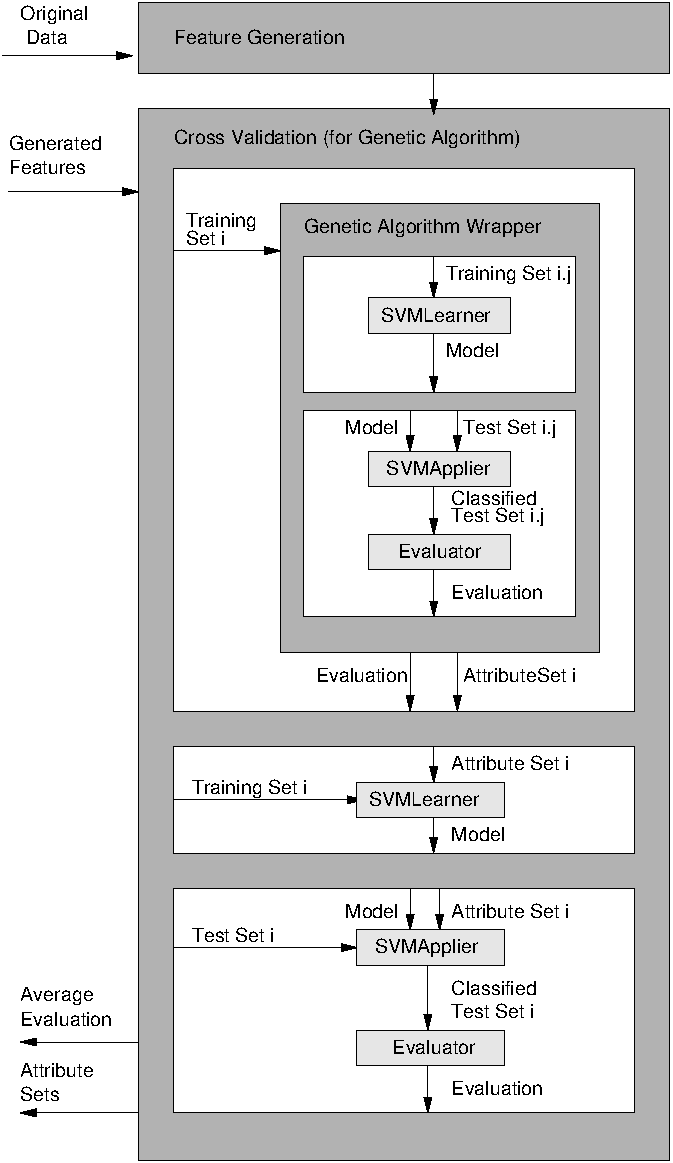
\includegraphics{graphics/genplusXValForGA.pdf}
  \caption[Feature selection using a genetic algorithm]{Nested operator chain for feature selection using a genetic algorithm.}
  \label{fig:methodvalidationchain_box}
\end{figure}





\section{\rapidminer as a Data Mining Interpreter}

\rapidminer uses XML (eXtensible Markup Language), a widely used language 
well suited for describing structured objects, to describe the
operator trees modeling KD processes.
   XML has become a standard format for data exchange.
Furthermore this format is easily readable by humans and machines. All
\rapidminer processes are described in an easy XML format. You can see this XML
description as a scripting language for data mining pocesses.

The graphical user interface and the XML based scripting language turn
\rapidminer into an IDE and interpreter for machine learning and data mining. Furthermore, the
XML process configuration files define a standardized interchange format
for data mining processes.




\section{Different Ways of Using \rapidminer}

\rapidminer can be started off-line, if the process configuration is provided
as XML file.
   Alternatively, the GUI of \rapidminer can be used to design the XML description
of the operator tree, to interactively control and inspect running processes, 
and to continuously monitor the visualization of the process results.
Break points can be used to check intermediate results and the data flow
between operators.
Of course you can also use \rapidminer from your program. Clear interfaces define an
easy way of applying single operators, operator chains, or complete operator
trees on you input data. A command line version and a Java API allows
invoking of \rapidminer from your programs without using the GUI. 
Since \rapidminer is entirely written in Java, it runs on any major
platform/operating system.




\section{Multi-Layered Data View Concept}
     

\rapidminer's most important characteristic is the ability to nest operator chains
and build complex operator trees. In order to support this characteristic the
\rapidminer data core acts like a data base management system and provides a
multi-layered data view concept on a central data table which underlies all
views. For example, the first view can select a subset of examples and the
second view can select a subset of features. The result is a single view which
reflects both views. Other views can create new attributes or filter the data
on the fly. The number of layered views is not limited.

This multi-layered view concept is also an efficient way to store different
views on the same data table. This is especially important for automatic data
preprocessing tasks like feature generation or selection. For example, the
population of an evolutionary operator might consist of several data views -
instead of several copies of parts of the data set. 
    
No matter whether a data set is stored in memory, in a file,
or in a database, \rapidminer internally uses a special type of data
table to represent it.
   In order not to unnecessarily copy the data set or subsets
of it, \rapidminer manages views on this table, so that only references
to the relevant parts of the table need to be copied or passed
between operators.
   These views are nestable as is for example required for nested
cross-validations by maintaining a stack of views.
   In case of an example set, views on the rows of the table 
correspond to subsets of the example set, and views on the
columns correspond to the selected features used to represent
these examples.




\section{Transparent Data Handling}

\rapidminer supports flexible process (re)arrangements which allows the search
for the best learning scheme and preprocessing for the data and learning task
at hand. The simple adaptation and evaluation of different process designs
allow the comparison of different solutions. 

\rapidminer achieves a transparent data handling by supporting several
types of data sources and hiding internal data transformations and
partitioning from the user. Due to the modular operator
concept often only one operator has to be replaced to evaluate its performance
while the rest of the process design remains the same. This is an important
feature for both scientific research and the optimization of real-world
applications.

The input objects of an operator may be consumed or passed on to 
following or enclosing operators. If the input objects are not required by
this operator, they are simply passed on, and may be used by later or outer 
operators.
This increases the flexibility of \rapidminer by easing the match of 
the interfaces of consecutive operators and allowing to pass objects
from one operator through several other operators to the goal operator.

Objects typically passed between operators are example sets, 
prediction models, evaluation vectors, etc.
Operators may add information to input objects, e.g. labels 
to previously unlabeled examples, or new features in a feature 
generation operator, and deliver these extended objects.




\section{Meta Data}

To guide the transformation of the feature space or the automatical search for
the best preprocessing, the user can define additional meta data on the data
set at hand. Meta data include the type of attributes or their unit (SI). This
information is for example used by the feature generation / construction
algorithms provided by \rapidminer. The definition of meta information on your data
is optional and if it is omitted \rapidminer tries to guess the correct data types.




\section{Large Number of Built-in Data Mining Operators}

\rapidminer provides more than 400 operators including:
\begin{description}
\item[Machine learning algorithms:] a huge number of learning schemes for
  regression and classification tasks including support vector machines (SVM),
  decision tree and rule learners, lazy learners, Bayesian learners, and
  Logistic learners. Several algorithms for association rule mining and
  clustering are also part of \rapidminer. Furthermore, we added several meta
  learning schemes including Bayesian Boosting.
\item[Weka operators:] all Weka operations like learning schemes and attribute
  evaluators of the Weka learning environment are also available and can be
  used like all other \rapidminer operators.
\item[Data preprocessing operators:] discretization, example and feature filtering,
  missing and infinite value replenishment, normalization, removal of useless
  features, sampling, dimensionality reduction, and more.
\item[Feature operators:] selection algorithms like forward selection,
  backward elimination, and several genetic algorithms, operators for feature
  extraction from time series, feature weighting, feature relevance, and
  generation of new features.
\item[Meta operators:] optimization operators for process design,
  e.g. example set iterations or several parameter optimization schemes.
\item[Performance evaluation:] cross-validation and other evaluation schemes,
  several performance criteria for classification and regression, operators
  for parameter optimization in enclosed operators or operator chains.
\item[Visualization:] operators for logging and presenting results. Create
  online 2D and 3D plots of your data, learned models and other process
  results.
\item[In- and output:] flexible operators for data in- and output, support of
several file formats including arff, C4.5, csv, bibtex, dBase, and reading
directly from databases.
\end{description}




\section{Extending \rapidminer}

\rapidminer supports the implementation of user-defined operators.
In order to implement an operator, the user simply needs to
define the expected inputs, the delivered outputs, the mandatory
and optional parameters, and the core functionality of the operator.
Everything else is done by \rapidminer. The operator description in XML
allows \rapidminer to automatically create corresponding GUI elements.
This is explained in detail in
chapter~\ref{sec:extending_rapidminer}. An easy-to-use plugin mechanism is provided
to add future operators or operators written by the \rapidminer community
into \rapidminer. Several plugins are already provided in the download
section of \rapidminer.

External programs can be integrated by implementing wrapper 
operators and can then be transparently used in any \rapidminer 
process.



\section{Example Applications}

\rapidminer has already been applied for machine learning and
knowledge discovery tasks in a number of domains including
feature generation and selection % to improve the classification and regression learning
\cite{Felske/etal/2003a,            %%  SFB-CI/C9-TR
      Klinkenberg/etal/2002a,       %%  FGML-2002
      Ritthoff/Klinkenberg/2003a,   %%  GECCO-2003
      Ritthoff/etal/2002b},         %%  UKCI-2002
concept drift handling
\cite{Klinkenberg/Joachims/2000a,   %%  ICML-2000
      Klinkenberg/2004a,
      Klinkenberg/2003a,
      Klinkenberg/Rueping/2003a},   %%  Daimler-WS-Buchkapitel
and transduction
\cite{Daniel/etal/2002a,            %%  SFB-CI-Ergebnisberichtbuchkapitel
      Klinkenberg/2001a}.           %%  IJCAI-2001-WS
In addition to the above-mentioned, current application domains of
\rapidminer also include
the pre-processing of and learning from time series
\cite{Mierswa/2004c,Mierswa/Morik/2005a,Mierswa/Morik/2005b},
meta learning \cite{Mierswa/Wurst/2005a,Mierswa/Wurst/2005b},
clustering, and text processing
and classification.  %% Word Vector Tool by Michael Wurst
There exist several plugins to provide operators for these special
learning tasks. Among these, there are some unusual plugins like GAStruct
which can be used to optimize the design layout for chemical plants
\cite{Mierswa/2005a,Mierswa/Geisbe/2004a}.


The Figures~\ref{fig:screen_experiment} and \ref{fig:screen_plot} 
show screenshots from two process definitions performed with the GUI version of \rapidminer.
   Figure~\ref{fig:screen_experiment} depicts the process tree and
the panel for setting the parameters of one of its operators in
a feature selection process using backward elimination as feature selector.
   Figure~\ref{fig:screen_plot} demonstrates the continuous result display
of a parameter optimization process.

\begin{figure}[ptbh]
  \center
    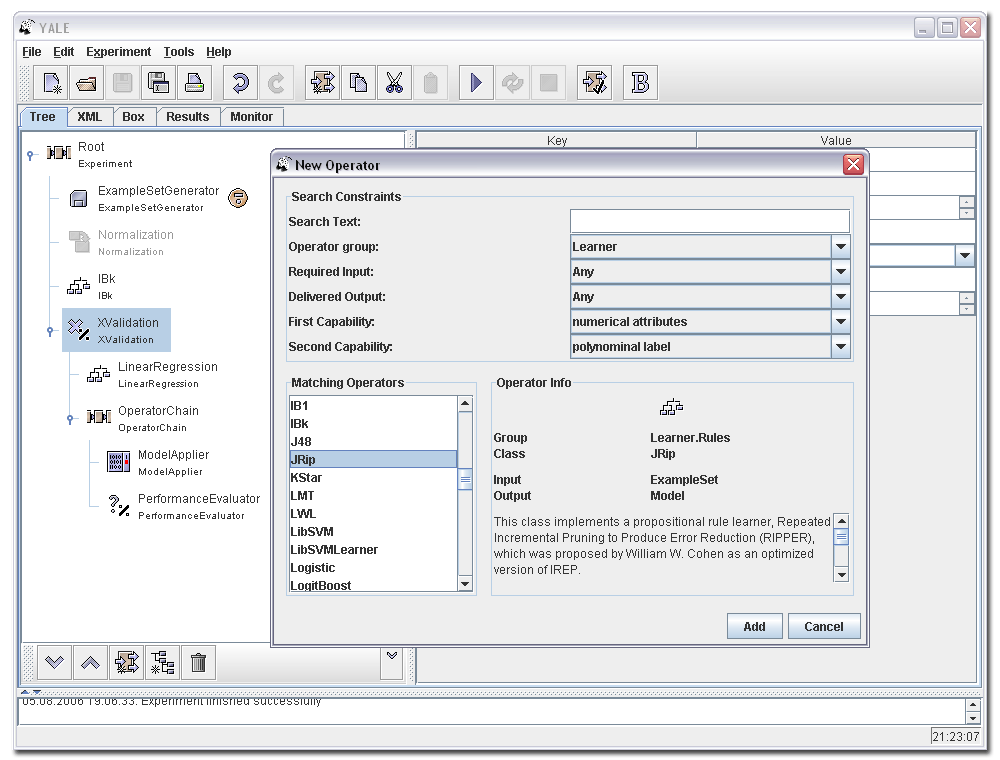
\includegraphics[height=0.4\textheight]{graphics/screenshots/screenshot_main1.png}
  \caption[\rapidminer GUI screenshot]{\rapidminer screenshot of the process tree and the panel for setting 
    the parameters of a feature selection operator.}
  \label{fig:screen_experiment}
\end{figure}

\begin{figure}[ptbh]
  \center
    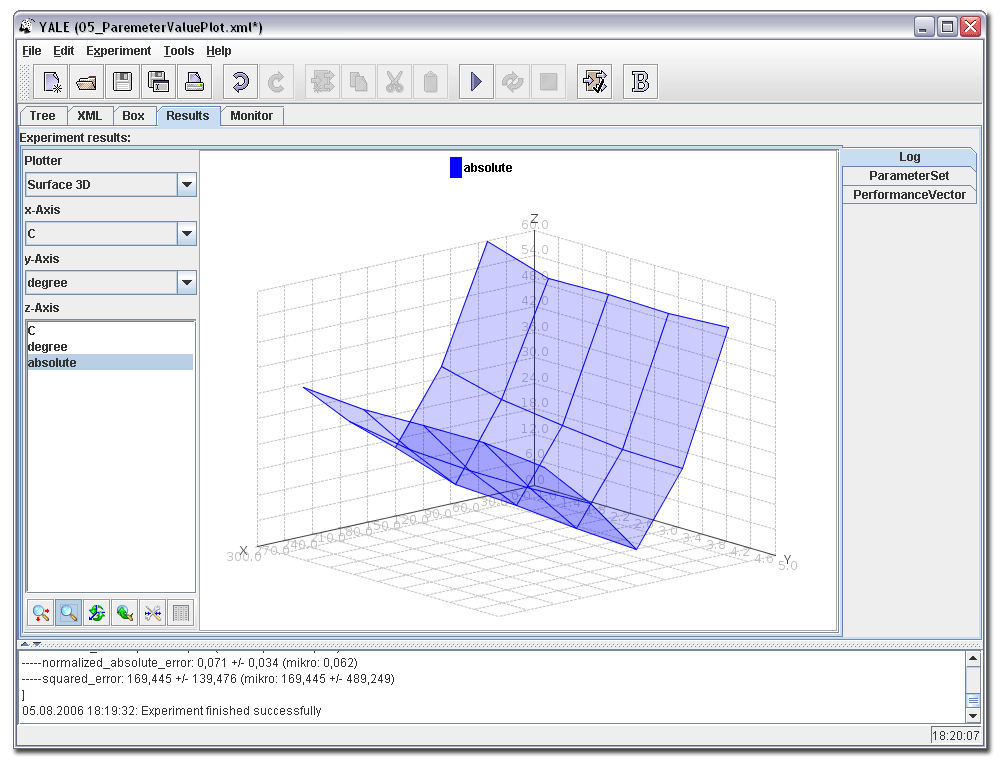
\includegraphics[height=0.4\textheight]{graphics/screenshots/screenshot_main2.png}
  \caption[Parameter optimization process screenshot]{\rapidminer screenshot of the continuous result display
    of a parameter optimization process.}
  \label{fig:screen_plot}
\end{figure}



\bigskip


Use \rapidminer and explore your data! Simplify the construction of data mining processes and
the evaluation of different approaches. Try to find the best combination of
preprocessing and learning steps or let \rapidminer do that automatically for
you. Have fun!




\section{How this tutorial is organized}

First you should read this chapter in order to get an idea of the concepts of
\rapidminer. Thereafter, we suggest that you read the GUI manual of \rapidminer
and make the online tutorial. It will be much easier to understand the
details explained in the next chapters. Chapter \ref{sec:first_steps}
describes possible first steps and the basics of \rapidminer. In Chapter
\ref{sec:advanced} we discuss more advanced processes. You should
read at least these two chapters to create your own
process setups. 
Chapter \ref{sec:operatorreference} provides information
about all \rapidminer core operators. It is an operator reference, i.e. you
can look up the details and description of all operators. 
Chapter \ref{sec:extending_rapidminer} can be omitted if you want to use
\rapidminer on your data or just want to perform some basic
process definitions. In this chapter we describe ways to extend \rapidminer by
writing your own operators or building own plugins.



\chapter{Installation and starting notes}

\section{Download}
The latest version of \rapidminer is available on the \rapidminer homepage:
\begin{quote}
  \rapidminerurl.
  \index{URL}
  \index{homepage}
\end{quote}
%
The \rapidminer homepage also contains this document, the \rapidminer javadoc, example
datasets, plugins, and example configuration files.

\section{Installation}
\index{installation}
\label{sec:installation}


This section describes the installation of \rapidminer on your machine. You may
install \rapidminer for all users of your system or for your own account 
locally.

Basically, there are two different ways of installing \rapidminer:
\begin{itemize}
\item Installation of a Windows executable
\item Installation of a Java version (any platform)
\end{itemize}

Both ways are described below. More information about the installation 
of \rapidminer can be found at \rapidminerurl.


\subsection{Installing the Windows executable}

Just perform a double click on the downloaded file 
\begin{verbatim}
     rapidminer-XXX-install.exe
\end{verbatim}
and follow the installation instructions. As a result, there will be
a new menu entry in the Windows startmenu. \rapidminer is started by clicking
on this entry.


\subsection{Installing the Java version (any platform)}

\rapidminer\ is completely written in Java, which makes it run on
almost every platform. Therefore it requires a Java Runtime
Environment (JRE) version 5.0 (aka 1.5.0) or 
higher to be installed properly. The runtime environment JRE is available at
\url{http://java.sun.com/}. It must be installed before \rapidminer can be installed.

In order to install \rapidminer, choose an installation directory and
unzip the downloaded archive using WinZIP or tar or similar programs:
\begin{verbatim}
> unzip rapidminer-XXX-bin.zip
\end{verbatim}
for the binary version or
\begin{verbatim}
> unzip rapidminer-XXX-src.zip
\end{verbatim}
for the version containing both the binaries and the sources.
This will create the \rapidminer home directory which contains the files
listed in table~\ref{tab:rapidminer_files}.

\begin{table}[hbtp]
  \begin{tabular}{ll}
    \hline
    \filename{etc/}                &       Configuration files\\
    \filename{lib/}                &       Java libraries and jar files\\
    \filename{lib/rapidminer.jar}  &       The core \rapidminer java archive\\
    \filename{lib/plugins}         &       Plugin files (Java archives)\\
    \filename{licenses/}           &       The GPL for \rapidminer and library licenses\\
    \filename{resources/}          &       Resource files (source version only)\\
    \filename{sample/}             &       Some sample processes and data\\
    \filename{scripts/}            &       Executables\\
    \filename{scripts/rapidminer}        & The commandline Unix startscript\\
    \filename{scripts/rapidminer.bat}    & The commandline Windows startscript\\
    \filename{scripts/RapidMinerGUI}     & The GUI Unix startscript\\
    \filename{scripts/RapidMinerGUI.bat} & The GUI Windows startscript\\
    \filename{src/}                &       Java source files (source version only)\\
    \filename{INSTALL}             &       Installation notes\\
    \filename{README}              &       Readme files for used libraries\\
    \filename{CHANGES}             &       Changes from previous versions\\
    \filename{LICENSE}             &       The GPL\\
    \hline
  \end{tabular}
  \caption{The \rapidminer directory structure.}
  \label{tab:rapidminer_files}
\end{table}


\section{Starting \rapidminer}

If you have used the Windows installation executable, you can start \rapidminer just
as any other Windows program by selecting the corresponding menu item from the
start menu.

On some operating systems you can start \rapidminer by double-clicking
the file \filename{rapidminer.jar} in the \filename{lib} subdirectory of \rapidminer. If
that does not work, you can type
\commandline{java -jar rapidminer.jar} on the command prompt. You can also use
the startscripts \filename{scripts/rapidminer} (commandline version) or
\filename{scripts/RapidMinerGUI} (graphical user interface version) for
Unix or \filename{scripts/\-rapidminer.bat} and \filename{scripts/\-RapidMinerGUI.bat} for
Windows.

If you intend to make frequent use of the commandline version of
\rapidminer, you might want to modify your local startup scripts adding the
\filename{scripts} directory to your \commandline{PATH}
environment variable. If you decide to do so, you can start a
process by typing \commandline{rapidminer <processfile>} from anywhere
on your system. If you intend to make frequent use of the GUI, you
might want to create a desktop link or a start menu item to
\filename{scripts/RapidMinerGUI} or \filename{scripts/RapidMinerGUI.bat}. Please refer to
your window manager documentation on information about this. Usually
it is sufficient to drag the icon onto the desktop and choose "`Create
link"' or something similar.

Congratulations: \rapidminer\ is now installed. In order to check if \rapidminer\ is
correctly working, you can go to the \filename{sample} subdirectory
and test your installation by invoking \rapidminer on the file
\filename{Empty.xml} which contains the simplest process setup that can
be conducted with \rapidminer. In order to do so, type
\begin{verbatim}
cd sample
rapidminer Empty.xml
\end{verbatim}
The contents of the file \filename{Empty.xml} is shown in
figure~\ref{fig:installation}. 
\examplefile{installtest.xml}{installation}{Installation test}

Though this process does, as you might guess, nothing,
you should see the message ``Process finished successfully'' after 
a few moments if everything goes well. Otherwise
the words "Process not successful" or another error message can be
read. In this case something is wrong with the installation.
Please refer to the Installation section of our website \rapidminerurl{} for further
installation details and for pictures describing the installation
process. 


\section{Memory Usage}
\label{sec:memory_usage}
\index{memory}

Since performing complex data mining tasks and machine learning methods on 
huge data sets might need a lot of main memory, it might be that \rapidminer stops
a running process with a note that the size of the main memory was not 
sufficient. In many cases, things are not as worse at this might sound at
a first glance. Java does not use the complete amount of available memory 
per default and memory must be explicitely allowed to be used by Java.

On the installation page of our web site \rapidminerurl{} you can find a description 
how the amount of memory usable by \rapidminer can be increased. This is, by the way, 
not necessary for the Windows executable of \rapidminer since the amount of available 
memory is automatically calculated and properly set in this case.



\section{Plugins}
\label{sec:plugins_installing}
\index{plugins!installing}

In order to install \rapidminer plugins, it is sufficient to copy them to the
\filename{lib/plugins} subdirectory of the \rapidminer installation
directory. \rapidminer scans all \filename{jar} files in this directory. In
case a plugin comes in an archive containing more than a single 
\filename{jar} file (maybe documentation or samples), please only
put the \filename{jar} file into the \filename{lib/plugins} directory and
refer to the plugin documentation about what to do with the other
files. For an introduction of how to create your own plugin, please
refer to section~\ref{sec:plugins_packaging} of this tutorial.

For Windows systems, there might also be an executable installer ending on
.exe which can be used to automatically install the plugin into the correct
directory. In both cases the plugin will become available after the next start
of \rapidminer.


 

\section{General settings}
\label{sec:globalsettings}
\index{settings}

During the start up process of \rapidminer you can see a list of configuration
files that are checked for settings. These are the files \filename{rapidminerrc} and
\filename{rapidminerrc.OS} where OS is the name of your operating system,
e.g. ``Linux'' or ``Windows 2000''. Four locations are scanned in
the following order
\begin{enumerate}
\item The \rapidminer home directory (the directory in which it is installed.)
\item The directory \filename{.rapidminer} in your home directory.
\item The current working directory.
\item Finally, the file specified by the java property
  \para{rapidminer.rcfile} is read. Properties can be passed to java by
  using the \commandline{-D} option: 
  \begin{verbatim}
java -Drapidminer.rcfile=/my/rapidminer/rcfile -jar rapidminer.jar
  \end{verbatim}
\end{enumerate}
Parameters in the home directory can override global parameters.
The most important options are listed in table \ref{tab:rapidminerrc_options} and take the
form \para{key=value}. Comments start with a \#. Users that are
familiar with the Java language recognize this file format as the Java
property file format.

A convenient dialog for setting these properties is available in the file menu
of the GUI version of \rapidminer.

\begin{table}[htbp]
  \newcolumntype{Y}{>{\small\raggedright\arraybackslash}X}
  \newcolumntype{Z}{>{\small\tt\raggedright\arraybackslash}l}
  \renewcommand{\tabularxcolumn}[1]{p{#1}}
  \begin{tabularx}{\linewidth}{|Z|Y|}
    \hline
    \textbf{Key}               & \textbf{Description} \\
    \hline\hline
    rapidminer.general.capabilities.warn &  indicates if only a warning should be shown if a learner does not have sufficient capabilities \\
    rapidminer.general.randomseed     & the default random seed \\
    \hline
    rapidminer.tools.sendmail.command&  the sendmail command to use for sending notification emails \\
    rapidminer.tools.gnuplot.command &  the full path to the gnuplot executable (for GUI only) \\
    rapidminer.tools.editor          &  external editor for Java source code \\
    \hline
    rapidminer.gui.attributeeditor.rowlimit & limit number of examples in attribute editor (for performance reasons) \\
    rapidminer.gui.beep.success      &  beeps on process success \\
    rapidminer.gui.beep.error        &  beeps on error \\
    rapidminer.gui.beep.breakpoint   &  beeps on reaching a breakpoint \\
    rapidminer.gui.processinfo.show & indicates if some information should be displayed after process loading \\
    %rapidminer.gui.messageviewer.highlight.errors & color for errors in the message viewer \\
    %rapidminer.gui.messageviewer.highlight.warnings & color for warnings in the message viewer \\
    %rapidminer.gui.messageviewer.rowlimit & limit number of lines in message viewer (for performance reasons) \\
    rapidminer.gui.plaf          & the pluggable look and feel; may be {\tt system}, {\tt cross\_{}platform}, or classname \\
    rapidminer.gui.plotter.colors.classlimit & limits the number of nominal values for colorized plotters, e.g. color histograms \\
    rapidminer.gui.plotter.legend.classlimit & limits the number of nominal values for plotter legends \\
    rapidminer.gui.plotter.matrixplot.size & the pixel size of plotters used in matrix plots \\
    rapidminer.gui.plotter.rows.maximum & limits the sample size of data points used for plotting \\
    rapidminer.gui.undolist.size & limit for number of states in the undo list \\
    rapidminer.gui.update.check & indicates if automatic update checks should be performed \\
    %rapidminer.gui.xml.highlight.main  & color for main keywords in the XML editor \\
    %rapidminer.gui.xml.highlight.other & color for other keywords in the XML editor \\
    %rapidminer.gui.xml.highlight.quote & color for quoted text in the XML editor \\
    \hline
  \end{tabularx}
  \caption{The most important rapidminerrc options.}
  \label{tab:rapidminerrc_options}
\end{table}



\section{External Programs}

The properties discussed in the last section are used to determine the
behavior of the \rapidminer core. Additionally to this, plugins can require names
and paths of executables used for special learning methods and
external tools. These paths are also defined as properties. The possibility of
using external programs such as machine learning methods is discussed in the
operator reference (chapter \ref{sec:operatorreference}). These programs must
have been properly installed and must be executable without \rapidminer, before they 
can be used in any \rapidminer process setup. By making use of the
\filename{rapidminerrc.OS} file, paths can be set in a platform dependent
manner.


\section{Database Access}
\label{sec:database_access}
\index{settings}
\index{jdbc}

It is very simple to access your data from a database management system like 
Oracle, Microsoft SQL Server, PostgreSQL, or mySQL. \rapidminer supports a wide range
of systems without any additional effort. If your database management system is 
not natively supported, you simply have to add the JDBC driver for your system to 
the directory \filename{lib/jdbc} or to your CLASSPATH variable.

If you want to ease the access to your database even further, you might think of 
defining some basic properties and description in the file
\begin{center} 
\filename{resources/jdbc\_properties.xml}
\end{center}
although this is not necessary to work on your databases and basically only eases
the usage of the database wizard for the convenient connection to your database
and query creation.


\chapter{First steps}
\label{sec:first_steps}

This chapter describes some basic concepts of \rapidminer. In the description, we assume that 
most of the processes are performed in batch mode (or command line mode). Of course you can also use \rapidminer in the
Graphical User Interface mode which is more convenient and offers a large
amount of additional features. A short documentation of the GUI mode
is separately available in the download section of the \rapidminer website.
\rapidminer provides an online tutorial which also describes the usage of the
GUI mode and the basic concepts of machine learning with \rapidminer.
Probably, you will not need to read all sections of this tutorial after making the
online tutorial and reading the short GUI manual. However, you should at least
read this section to get a first idea about some of the \rapidminer concepts.

All examples described in this tutorial are part of the sample directories of
\rapidminer. Although only few of these examples are discussed here, you should take
a look at all of them since they will give you some helpful hints. We
suggest that you start approximately the first half of the process definitions in each
of the sample directories in the order the directories are named, i.e. first
the first half of directory \filename{01\_IO}, then the first half of \filename{02\_Learner} and so
on. After this round, you should again start with the first directory and
perform the second half of the process setups. This way the more complicated
processes will be performed after you had a look at almost all of the simple
building blocks and operators.

\section{First example}
\label{sec:firstexample}
\index{example processes!simple}


Let us start with a simple example \filename{03\_XValidation\_Numerical.xml} which
you can find in the \filename{04\_Validation} subdirectory. This example process loads an example set
from a file, generates a model using a support vector machine (SVM)
and evaluates the performance of the SVM on this dataset by estimating
the expected absolute and squared error by means of a ten-fold
cross-validation. In the following we will describe what the
parameters mean without going into detail too much. We will describe
the used operators later in this section.

\examplefileshort{simpleexample.xml}{simpleexample}{Simple example
  configuration file. This is the \filename{03\_XValidation\_Numerical.xml} sample process}{Simple example
  configuration file}

But first of all let's start the process. We assume that your
current folder contains the file \filename{03\_XValidation\_Numerical.xml} (see
figure \ref{fig:simpleexample}). Now start \rapidminer by typing
\begin{verbatim}
rapidminer 03_XValidation_Numerical.xml
\end{verbatim}
or by opening that file with the
GUI and pressing the start button. After a short while you should
read the words ``Process finished successfully''. Congratulations,
you just made your first \rapidminer process. If you read ``Process
not successful'' instead, something went wrong. In either case you
should get some information messages on your console (using \rapidminer in batch mode) or
in the message viewer (GUI mode). In the latter case it should give
you information about what went wrong. All kinds of debug messages as
well as information messages and results like the calculated relative
error are written to this output. Have a look at it now.

The log message starts with the process tree and contains a lot of
warnings, because most of the parameters are not set. Don't panic,
reasonable default values are used for all of them. At the end, you will
find the process tree again. The number in squared brackets
following each operator gives the number of times the operator was
applied. It is one for the outer operators and ten within the ten-fold
cross-validation. Every time an operator is applied a message is written
to the log messages indicating its input objects (like example sets and
models). When the operator terminates its application it writes the
output to the log stream again. You can find the average performance
estimated by the cross-validation close to the end of the messages.

Taking a look at the process tree in the log messages once again, you
will quickly understand how the configuration file is structured. 
There is one \tag{operator} tag for each operator specifying its 
name and class. Names must be unique and have the only purpose of 
distinguishing between instances of the same class.
Operator chains like the cross-validation chain may contain one 
or more inner operators. Parameters can be specified in the form of
key-value pairs using a \tag{parameter} tag.

We will now focus on the operators without going into detail too
much. If you are interested in the the operator classes, their input
and output objects, parameters, and possible inner operators you may
consult the reference section of this tutorial 
(chapter \ref{sec:operatorreference}). 

The outermost operator called ''Root'' is a
\op{Process} operator, a subclass of a simple \op{OperatorChain}. An
operator chain works in a very simple manner. It applies its inner
operators successively passing their respective output to the next
inner operator. The output of an operator chain is the output of the
last inner operator. While usual operator chains do not take any
parameters, this  particular operator chain (being the outermost
operator) has some parameters that are important for the process as
a whole, e.g. the name of the log file (\para{logfile}) and the name
of the directory for temporary files ({\para{temp\_dir}).

The \op{ExampleSource} operator loads an example set from a file. An
additional file containing the attribute descriptions is
specified (\filename{data/polynomial.xml}). References to the actual data
files are specified in this file as well (see section
\ref{sec:inputfiles} for a description of the files). Then the resulting
example set is passed to the cross-validation chain.

The \op{XValidation} evaluates the learning method by splitting 
the input example set into ten subsets $S_{1},\ldots,S_{10}$. 
The inner operators are applied ten times.  In run number $i$ the
first inner operator, which is a \op{LibSVMLearner}, generates a model
using the training set $\bigcup_{j \neq i} S_{j}$. The second inner
operator, an evaluation chain, evaluates this model by applying it to
the remaining test set $S_{i}$. The \op{ModelApplier} predicts labels
for the test set and the \op{PerformanceEvaluator} compares them to
the real labels. Afterwards the absolute and squared errors are
calculated. Finally the cross-validation chain returns the average
absolute and squared errors over the ten runs and their variances.

The processing of \rapidminer operator trees is similar to a depth first search of
normal trees. In contrast to this usual way of traversing a tree, \rapidminer allows
loops during the run (each learning child is used 10 times, the applier chain
is used 10 times, too). Additionally, inner nodes may perform some operations
before they pass the output of the first children to the next child. The
traversal through a \rapidminer operator tree containing leaf operators and simple
operator chains only is actually equivalent to the usual depth first search
traversal.



\section{Process configuration files}
\index{configuration file}
\label{configuration_file}

Process configuration files are XML documents containing only four types
of tags (extension: \filename{.xml}). If you use the GUI version of \rapidminer, you can display the
configuration file by clicking on the XML tab. Process files define
the process tree consisting of operators and the parameters for
these operators. Parameters are single values or
lists of values. Descriptions can be used to comment your operators.

\subsection*{$<$operator$>$}
The \tag{operator} tag represents one instance of an operator
class. Exactly two attributes must be present:
\begin{description}
\item [name:] A unique name identifying this particular operator instance
\item [class:] The operator class. See the operator reference (chapter
\ref{sec:operatorreference}) for a list of operators.
\end{description}
For instance, an operator tag for an operator that reads an example
set from a file might look like this:\smallskip

\begin{lstlisting}[style=rapidminerxmlstyle]{}
<operator name="MyExampleSource" class="ExampleSource">
</operator>
\end{lstlisting}

\noindent
If \tag{class} is a subclass of \op{OperatorChain}, then nested
operators may be contained within the opening and closing
tag.


\subsection*{$<$parameter$>$ and $<$list$>$}
As discussed above, a parameter can have a single value or a set of
values. For single value parameters the \tag{<parameter>} tag is used. The
attributes of the \tag{<parameter>} tag are as follows:
\begin{description}
\item[key:] The unique name of the parameter.
\item[value:] The value of the parameter. 
\end{description}

In order to specify a filename for the example above, there might be used the
following parameter:
\bigskip

\begin{lstlisting}[style=rapidminerxmlstyle]{}
<operator name="MyExampleSource" class="ExampleSource">
  <parameter key="attributes" value="myexamples.dat"/>
</operator>
\end{lstlisting}

If the parameter accepts a list of values, the \tag{<list>} tag must be
used. The list must have a \tag{key} attribute, just as the
\tag{<parameter>} tag. The elements of the list are specified by nested
\tag{<parameter>} tags, e.g. in case of a \op{FeatureGeneration}
operator (see section \ref{sec:op:FeatureGeneration}).
\bigskip

\begin{lstlisting}[style=rapidminerxmlstyle]{}
<list key="functions">
  <parameter key="sum"     value="+(a1,a2)"/>
  <parameter key="product" value="*(a3,a4)"/>
  <parameter key="nested"  value="+(*(a1,a3),a4)"/>
</list>
\end{lstlisting}



\subsection*{$<$description$>$}
All operators can have an inner tag named \tag{<description>}. It has
only one attribute named \tag{text}. This attribute contains a comment
for the enclosing operator. If the root operator of the process has
an inner description tag, the text is displayed after loading the
process setup.

\begin{lstlisting}[style=rapidminerxmlstyle]{}
<operator name="MyExampleSource" class="ExampleSource">
  <description text="Loads the data from file." />
</operator>
\end{lstlisting}


\section{Parameter Macros}
\label{parameter_macros}

All text based parameters might contain so called macrors which will be replaced
by \rapidminer during runtime. For example, you can write a learned model into a file 
with the operator \op{ModelWriter} (see \ref{sec:op:ModelWriter}). If you want to do
this for each learned model in a cross validation run, each model would be overwritten
by the next one. How can this be prevented?

To save all models for each iteration in an own file, you need parameter macros.
In a parameter value, the character '\%' has a special meaning. Parameter values 
are expanded as follows:

  \begin{description}
  \item[\%\{a\}] is replaced by the number of times the operator was
  applied.
  \item[\%\{b\}] is replaced by the number of times the operator was
  applied plus one, i.e. $\%\textrm{a} + 1$. This is a shortcut for \%p[1].
  \item[\%\{p[number]\}] is replaced by the number of times the operator was
  applied plus the given number, i.e. $\%\textrm{a} + number$.
  \item[\%\{t\}] is replaced by the system time.
  \item[\%\{n\}] is replaced by the name of the operator.
  \item[\%\{c\}] is replaced by the class of the operator.
  \item[\%\{\%\}] becomes \%.
  \item[\%\{process\_name\}] becomes the name of the process file (without path and extension).
  \item[\%\{process\_file\}] becomes the name of the process file (with extension).
  \item[\%\{process\_path\}] becomes the path of the process file.
  \end{description}

For example to enumerate your files with ascending numbers, please use the following
value for the \tag{key} \para{model-file}: 

\begin{lstlisting}[style=rapidminerxmlstyle]{}
<operator name="ModelWriter" class="ModelWriter">
  <parameter key="model_file"	value="model_%{a}.mod"/>
</operator>
\end{lstlisting}

The macro \%\{a\} will be replaced by the number of times the operator was applied, 
in case of model write after the learner of a 10-fold cross validation it will hence
be replaced by the numbers 1 to 10.

You can also define own macros with help of the \op{MacroDefinition} operator 
(see \ref{sec:op:MacroDefinition}).



\section{File formats}
\label{sec:inputfiles}

\rapidminer can read a number of input files. Apart from data files it can
read and write models, parameter sets and attribute sets. Generally, \rapidminer
is able to read all files it generates. Some of the file formats are
less important for the user, since they are mainly used for intermediate
results. The most important file formats are those for ``examples'' or
``instances''. These data sets are provided by the user and almost all
processes contain an operator that reads them.


\subsection{Data files and the attribute description file}
\label{attribute_description_file}

If the data files are in the popular arff format (extension:
\filename{.arff}), which provides some meta data,
they can be read by the \refop{ArffExampleSource}. Other operators for
special file formats are also available. Additionally, data can be read from a
data base using the \refop{DatabaseExampleSource}. In that case, meta data is
read from the data base as well.

The \op{ExampleSource} operator allows for a variety of other file formats in
which instances are separated by newline characters. It is the main data input
operator for \rapidminer. Comment characters can be 
specified arbitrarily and attributes can be spread
over several files. This is especially useful in cases where attribute data and
the label are kept in different files.

Sparse data files can be read using the
\op{SparseFormat\-ExampleSource}. We call data sparse if almost all values are
equal to a default, e.g. zero.

The \op{ExampleSource} (for dense data) and some sparse formats
need an attribute description file (extension: \filename{.aml}) in order to
retrieve meta data about the instances. This file is a simple XML document
defining the properties of the attributes (like their name and range) and
their source files. The data may be spread over several files. Therefore, the
actual data files do not have to be specified as a parameter of
the input operator.

The outer tag must be an \tag{<attributeset>} tag. 
The only attribute of this tag may be \tag{default\_source=}\para{filename}.
This file will be used as a default file if it is not specified
explicitly with the attribute.

The inner tags can be any number of \tag{<attribute>} tags plus at
most one tag for each special attribute. The most frequently used
special attributes are \tag{<label>}, \tag{<weight>}, \tag{<id>}, and \tag{<cluster>}. 
Note that arbitrary names for special attributes may be
used. Though the set of special attributes used by the core \rapidminer
operators is limited to the ones mentioned above, plugins or
any other additional operators may use more special attributes. Please
refer to the operator documentation to learn more about the specific
special attributes used or generated by these operators.

The following XML attributes may be set to specify the properties of
the \rapidminer attribute declared by the corresponding XML tag 
(mandatory XML attributes are set in italic font):
\begin{description}
\item[\textit{name:}] The unique name of the attribute.
\item[sourcefile:] The name of the file containing the data.
  If this name is not specified, the default file is used (specified for
  the parent \tag{attributeset} tag).
\item[\textit{sourcecol:}] The column within this file (numbering starts
  at 1). Can be omitted for sparse data file formats.
\item[sourcecol\_end:] If this parameter is set, its value must be
  greater than the value of \tag{sourcecol}. In that case,
  $sourcecol-sourcecol\_end$ attributes are generated with the same
  properties. Their names are generated by appending numbers to the
  value of \tag{name}. If the \tag{blocktype} is
  \parval{value\_series}, then \parval{value\_series\_start} and
  \parval{value\_series\_end} respectively are used for the first and
  last attribute blocktype in the series.
\item[\textit{valuetype:}] One out of \parval{nominal}, \parval{numeric},
  \parval{integer}, \parval{real}, \parval{ordered}, \parval{binominal},
  \parval{polynominal}, and \parval{file\_path}
\item[blocktype:] One out of \parval{single\_value},
  \parval{value\_series}, \parval{value\_series\_start},
  \parval{value\_series\_end}, \parval{interval},
  \parval{interval\_start}, and \parval{interval\_end}.
\end{description}

Each \textit{nominal} attribute, i.e. each attribute with a nominal (binominal, polynominal) 
value type definition, should define the possible values with help of inner tags 
\begin{center}
\tag{<value>}nominal\_value\_1\tag{</value>} \\
\tag{<value>}nominal\_value\_2\tag{</value>} \\
\ldots
\end{center}

See figure \ref{fig:attributefile} for an example attribute
description file. 
For classification learners that can handle only binary classifications 
(e.g. ``yes'' and ``no'') the first defined value in the list of nominal values
is assumed to be the negative label. That includes the classification ``yes''
is not necessarily the positive label (depending on the order). This is important,
for example, for the calculation of some performance measurements like
precision and recall.

\examplefile{attributes.xml}{attributefile}{An example attribute set description file in XML syntax.}

\textit{Note:} Omitting the inner value tags for nominal attributes
will usually \textit{seem} to work (and indeed, in many cases no problems might
occur) but since the internal representation of nominal values depend on this
definition it might happend that the nominal values of learned models do not fit 
the given data set. Since this might lead to drastically reduced prediction accuracies
you should always define the nominal values for nominal attributes.

\textit{Note:} You do not need to specify a label
attribute in cases where you only want to predict a label with a learned
model. Simply describe the attributes in the same manner as in the learning
process setup, the label attribute can be omitted.


\subsubsection{Dense data files}
\index{attribute set description file}
The data files are in a very simple format (extension: \filename{.dat}). By default,
comments start with \#. When a comment character is encountered, the
rest of the line is discarded. Empty lines -- after comment removal
-- are ignored. If the data is spread over several files, a non empty
line is read from every file. If the end of one of the files is
reached, reading stops. The lines are split into tokens that are 
whitespace separated by default, separated by a comma, or separated by semicolon. The number of the tokens are mapped to
the \tag{sourcecol} attributes specified in the attribute description
file. Additional or other separators can be specified as a regular expression
using the respective parameters of the \refop{ExampleSource}. 
The same applies for comment characters.


\subsubsection{Sparse data files}
\label{sec:sparse_format}
If almost all of the entries in a data file are zero or have a default nominal
value, it may be well suitable to use a \refop{SparseFormatExampleSource}. This
operator can read an attribute description file as described above. If the
\para{attribute\_description\_file} parameter is supplied, the attribute
descriptions are read from this file and the \tag{default\_source} is used as
the single data file. The \tag{sourcecol} and \tag{sourcefile} attributes are
ignored. If the \para{attribute\_description\_file} parameter is not supplied,
the data is read from the file \para{data\_file} and attributes are generated
with default value types. Regular attributes are supposed to be real numbers
and the label is supposed to be nominal. In that case, the \para{dimension}
parameter, which specifies the number of regular attributes, must be set.

Comments in the data file start with a '\#'-character, empty lines are
ignored. Lines are split into whitespace separated tokens of the form
\filecont{index:value} where \para{value} is the attribute value,
i.e. a number or a string, and \para{index} is either an index number
referencing a regular attribute or a prefix for a special attribute
defined by the parameter list \para{prefix\_map} of the
\op{SparseFormatExampleSource}. Please note that index counting starts with 1.


The \op{SparseFormatExampleSource} parameter \para{format} specifies
the way labels are read.
\begin{description}
\item[xy] The label is the last token in the line.
\item[yx] The label is the first token in the line.
\item[prefix] The label is treated like all other special attributes.
\item[separate\_file] The label is read from a separate file. In that case,
  parameter \para{label\_file} must be set.
\item[no\_label] The example set is unlabeled.
\end{description}

All attributes that are not found in a line are supposed to have default
values. The default value for numerical data is 0, the default vallue for nominal
attributes is the first string specified by the \tag{classes} attribute in the
attribute description file.

\paragraph{Example} Suppose you have a sparse file which looks like
this:
\begin{verbatim}
w:1.0 5:1   305:5 798:1 yes
w:0.2 305:2 562:1       yes
w:0.8 49:1  782:1 823:2 no
...
\end{verbatim}
You may want each example to have a special attribute ``weight'', a
nominal label taking the values ``yes'' and ``no'', and 1\,000 regular
numerical attributes. Most of them are 0. The best way to read this
file, is to use a \op{SparseFormatExampleSource} and set the parameter
value of \para{format} to \parval{xy} (since the label is the last
token in each line) and use a \para{prefix\_map} that maps the prefix
``w'' to the attribute ``weight''. See figure~\ref{fig:sparse_format}
for a configuration file.
\examplefile{sparseformat.xml}{sparse_format}{Configuration of a \op{SparseFormatExampleSource}}



\subsection{Model files}
\index{model file}
Model files contain the models generated by learning operators in 
previous \rapidminer runs (extension: \filename{.mod}). Models can be written to a file by using the operator
\op{ModelWriter}. They can be read by using a \op{ModelLoader} and applied
by using a \op{ModelApplier}.



\subsection{Attribute construction files}
\label{sec:attributegenerationfiles}
\index{attribute set description file}
An \op{AttributeConstructionsWriter} writes an attribute set to a text file
(extension: \filename{.att}). 
Later, this file can be used by an \op{AttributeConstructionsLoader} operator
to generate the same set of attributes in another process and/or
for another set of data.

The attribute generation files can be generated by hand as well. Every
line is of the form
 
\begin{lstlisting}[style=rapidminerxmlstyle]{}
<attribute name="attribute_name" construction="generation_description"/>
\end{lstlisting}

The generation description is defined by functions, with prefix-order
notation. The functions can be nested as well. An example
of a nested generation description might be: $f(g(a), h(b), c)$. See
page \ref{sec:op:FeatureGeneration} for a reference of the available
functions.

Example of an attribute constructions file:

\begin{lstlisting}[style=rapidminerxmlstyle]{}
<constructions version="4.0">
    <attribute name="a2" construction="a2"/>
    <attribute name="gensym8" construction="*(*(a1, a2), a3)"/>
    <attribute name="gensym32" construction="*(a2, a2)"/>
    <attribute name="gensym4" construction="*(a1, a2)"/>
    <attribute name="gensym19" construction="*(a2, *(*(a1, a2), a3))"/>
</constructions>
\end{lstlisting}




\subsection{Parameter set files}
\label{sec:parameter_set_files}
For example, the \op{GridParameterOptimization} operator generates a set of optimal
parameters for a particular task (extension: \filename{.par}). Since parameters of several
operators can be optimized at once, each line of the parameter set
files is of the form
\begin{verbatim}
OperatorName.parameter_name = value
\end{verbatim}
These files can be generated by hand as well and can be read by a
\op{ParameterSetLoader} and set by a \op{ParameterSetter}.


\subsection{Attribute weight files}
\label{sec:attribute_weight_files}
All operators for feature weighting and selection generate a set of feature
weights (extension: \filename{.wgt}). Attribute selection is seen as attribute weighting which allows more
flexible operators. 
For each attribute the weight is stored, where a weight of 0 means
that the attribute was not used at all. For writing the files to a
file the operator \op{AttributeWeightsWriter} can be used. In such a
weights file each line is of the form
\begin{verbatim}
<weight name="attribute_name" value="weight"/>
\end{verbatim}
These files can be generated by hand as well and can be read by an
\op{AttributeWeightsLoader} and used on example sets with the operator
\op{AttributeWeightsApplier}. They can also be read and adapted with the
\op{InteractiveAttributeWeighting} operator.
Feature operators like forward selection, genetic algorithms and the weighting
operators can deliver an example set with the selection / weighting already
applied or the original example set (optional). In the latter case the weights
can adapted and changed before they are applied.

Example of an attribute weight file:
\begin{lstlisting}[style=rapidminerxmlstyle]{}
<attributeweights version="4.0">
    <weight name="a1" value="0.8"/>
    <weight name="a2" value="1.0"/>
    <weight name="a3" value="0.0"/>
    <weight name="a4" value="0.5"/>
    <weight name="a5" value="0.0"/>
</attributeweights>
\end{lstlisting}


\section{File format summary}

Table \ref{tab:file_extension} summarizes all file formats and the
corresponding file extensions.

\begin{table}[htbp]
  \newcolumntype{Y}{>{\small\raggedright\arraybackslash}X}
  \newcolumntype{Z}{>{\small\tt\raggedright\arraybackslash}l}
  \renewcommand{\tabularxcolumn}[1]{p{#1}}
  \begin{tabularx}{\linewidth}{|Z|Y|}
    \hline
    \textbf{Extension}               & \textbf{Description} \\
    \hline
    \filename{.aml} & attribute description file (standard XML meta data format) \\
    \filename{.arff}& attribute relation file format (known from Weka) \\
    \filename{.att} & attribute set file \\
    \filename{.bib} & BibTeX data file format \\
    \filename{.clm} & cluster model file (clustering plugin) \\
    \filename{.cms} & cluster model set file (clustering plugin) \\
    \filename{.cri} & population criteria file \\
    \filename{.csv} & comma separated values data file format \\
    \filename{.dat} & (dense) data files \\
    \filename{.ioc} & IOContainer file format \\
    \filename{.log} & log file / process log file \\
    \filename{.mat} & matrix file (clustering plugin) \\
    \filename{.mod} & model file \\
    \filename{.obf} & obfuscation map\\
    \filename{.par} & parameter set file \\
    \filename{.per} & performance file \\
    \filename{.res} & results file \\
    \filename{.sim} & similarity matrix file (clustering plugin) \\
    \filename{.thr} & threshold file \\
    \filename{.wgt} & attribute weight file \\
    \filename{.wls} & word list file (word vector tool plugin) \\
    \filename{.xrff}& extended attribute relation file format (known from Weka) \\
    \hline
  \end{tabularx}
  \caption{The most important file formats for \rapidminer.}
  \label{tab:file_extension}
\end{table}



\chapter{Advanced processes}
\label{sec:advanced}
\index{example processes!advanced}

At this point, we assume that you are familiar with the simple example 
from section \ref{sec:firstexample}. 
You should know how to read a dataset from a file, what a learner and 
a model applier do, and how a cross-validation chain works.
These operators will be used frequently and without further explanation
in this chapter. After reading this chapter you should be able to understand
most of the sample process definitions provided in the \filename{sample} directory of
\rapidminer. You should have a look at these examples and play around to get
familiar with \rapidminer.



\section{Feature selection}
\label{sec:advanced_feature_selection}
\index{feature selection}
Let us assume that we have a dataset with numerous attributes. 
We would like to test, whether all of these attributes are really
relevant, or whether we can get a better model by omitting some of 
the original attributes.
This task is called {\em feature selection} and the 
{\em backward elimination} algorithm is an approach that can 
solve it for you. 

Here is how backward elimination works within \rapidminer:
Enclose the cross-validation chain by a \op{FeatureSelection} 
operator. This operator repeatedly applies the cross-validation chain,
which now is its inner operator, until the specified stopping
criterion is complied with. The backward elimination approach
iteratively removes the attribute whose removal yields the largest
performance improvement. The stopping criterion may be for example 
that there has been no improvement for a certain number of steps. See
section \ref{sec:op:FeatureSelection} for a detailed description of
the algorithm. Figure \ref{fig:advanced1} shows the configuration
file.

You should try some of the following things:

\begin{itemize}
  \item Use {\em forward selection} instead of backward elimination by
    changing the parameter value of \para{selection\_direction} from
    \parval{backward} to \parval{forward}.
    This approach starts with an empty attribute set and iteratively
    adds the attribute whose inclusion improves the performance the
    most.
  \item Use the \op{GeneticAlgorithm} operator for feature selection
    instead of the \op{FeatureSelection} operator (see section
    \ref{sec:op:GeneticAlgorithm}).
  \item Replace the cross validation by a filter based evaluation. The sample
  process \filename{FeatureSelectionFilter.xml} uses such a fast feature
  set evaluation.
  \item Compare the results of the three approaches above to the 
    \op{BruteForce} operator.
    The brute force approach tests all subsets of the original attributes,
    i.e. all combinations of attributes, to select an optimal subset.
    While this operator is prohibitively expensive for large attribute
    sets, it can be used to find an optimal solution on small attribute 
    sets in order to estimate the quality of the results of other
    approaches.
\end{itemize}

\examplefile{advanced1.xml}{advanced1}{A feature selection process}




\section{Splitting up Processes}
\index{model file}
\index{attribute set description file}
If you are not a computer scientist but a data mining user, you are
probably interested in a real-world application of \rapidminer. 
   May be, you have a small labeled dataset and would like to train
a model with an optimal attribute set. 
   Later you would like to apply this model to your huge unlabeled 
database.
   Actually you have two separate processes.

\subsection{Learning a model}
This phase is basically the same as described in the preceeding section.
   We append two operators to the configuration file that write the results
of the process into files.
   First, we write the attribute set to the file 
\filename{selected\_at\-tri\-butes.att} using an \op{AttributeSetWriter}.
   Second, we once again train a model, this time using the entire example
set, and we write it to the file \filename{model.mod} with help of a
   \op{ModelWriter}.
   For the configuration file see figure \ref{fig:advanced2}. 
Execute the process and take a look at the file \filename{attributes.att}.
It should contain the selected subset of the originally used attributes, 
one per line.

\examplefile{advanced2.xml}{advanced2}{Training a model and writing it
to a file}

\subsection{Applying the model}
In order to apply this learned model to new unlabeled dataset, you
first have to load this example set as usual using an \op{ExampleSource}.
   You can now load the trained model using a \op{ModelLoader}.
Unfortunately, your unlabeled data probably still uses the original 
attributes, which are incompatible with the model learned on the
reduced attribute set.
   Hence, we have to transform the examples to a representation
that only uses the selected attributes, which we saved to the file 
\filename{attributes.att}.
   The \op{AttributeSetLoader} loads this file and generates (or rather
selects) the attributes accordingly.
   Now we can apply the model and finally write the labeled data 
to a file.
See figure \ref{fig:advanced3} for the corresponding configuration file. 

As you can see, you can easily use different dataset source files even in
different formats as long as you use consistent names for the attributes. 
You could also split the process into three parts:
\begin{enumerate}
  \item Find an optimal attribute set and train the model.
  \item Generate or select these attributes for the unlabeled data and
    write them to temporary files.
  \item Apply the model from step one to the temporary files from step
    two and write the labeled data to a result file.
\end{enumerate}

Of course it is also possible to merge all process modules into one big
process definition.

\examplefile{advanced3.xml}{advanced3}{Applying the model to unlabeled
data}




\section{Parameter and performance analysis}
\index{analysis}
\label{sec:parameter_optimization}
In this section we show how one can easily record performance values
of an operator or operator chain depending on parameter values. 
In order to achieve this, the \rapidminer process setup described in
this section makes use of two new \rapidminer operators: 
\refop{GridParameterOptimization} and \refop{ProcessLog}.

We will see how to analyze the performance of a support vector machine
(SVM) with a polynomial kernel depending on the two parameters 
degree $d$ and $\varepsilon$.\footnote{The performance of a polynomial
SVM also depends on other parameters like e.g. $C$, but this is not
the focus of this process.}

We start with the building block we should now be familiar with: a validation
chain containing a \op{LibSVMLearner}, a \op{ModelApplier}, and a
\op{PerformanceEvaluator}. Now we would like to vary the parameters.

Since we want to optimize more than one parameter, we cannot pass this
information to the \op{GridParameterOptimization} operator using the usual
\tag{<parameter>} tag. As the latter is designed to take a single
value, we must use the \tag{<list>} tag, which can take several
parameters. Similar to the \tag{<parameter>} tag the \tag{<list>} tag
must have a key. In case of the \op{GridParameterOptimization} this key is
(slightly confusingly in this context) named \para{parameters} (the
list of parameters which should be optimized). Each parameter 
that might be optimized, needs a \tag{<parameter>} tag entry in the \tag{<list>}.
The \tag{key} of a  \tag{<parameter>} tag has the form
\parval{OperatorName.parameter\_name} and the \tag{value} is a comma
separated list of values. In our case, the operator is named
"Training" and the parameters are \para{degree} and
\para{epsilon}. This leads to the following xml fragment:
\medskip

\begin{lstlisting}[style=rapidminerxmlstyle]{}
<list key="parameters">
  <parameter key="Training.degree" value="1,2,3,4"/>
  <parameter key="Training.epsilon" value="0.01,0.03,0.05,0.1"/>
</list>
\end{lstlisting}

Figure \ref{fig:advanced4} shows the entire example process setup.

\examplefile{advanced4.xml}{advanced4}{Parameter and performance analysis}

In GUI mode you do not have to bother about the XML code, just click
on the \useroption{Edit List} button next to the \para{parameters}
parameter of the \op{GridParameterOptimization} operator and add the two
parameters to the list.

If the value lists hold $n_1$ and $n_2$ values, respectively, the
\op{GridParameterOptimization} will apply its inner operators $n_1\cdot
n_2$ times. Finally the \op{GridParameterOptimization} operator returns an
optimal parameter value combination and the best performance
vector. If this is desired, the optimal parameter set can be written
to a file (for a specification see section
\ref{sec:parameter_set_files}) and reread from another process
using a \refop{ParameterSetLoader} and set using a
\refop{ParameterSetter}.
\medskip

In order to create a chart showing the absolute error over the parameters
$d$ and $\varepsilon$, we use the \op{ProcessLog} operator. Each time
this operator is applied, it creates a record containing a set of data
that we can specify. If the operator is applied $n$ times and we
specify $m$ parameters, we have a table with $n$ rows and $m$ columns
at the end of the process. Various plots and charts may be
generated from this table.

Similar to the optimization operator, the \op{ProcessLog} operator
accepts a \tag{<list>} of parameters specifying the values that should
be recorded. This list has the key \para{log}.
In our case, we are interested in three values: the values
of the parameters \para{degree} and \para{epsilon} and in the
performance of the models generated with these parameters. Therefore,
we add one \tag{<parameter>} tag to the \para{log} parameter
\tag{<list>} for each value we are interested in. (Again, in GUI mode,
simply click on the \useroption{Edit List} button next to the
\para{log} parameter of the \op{ProcessLog} operator.) The keys of
the parameters nested in this list may have arbitrary values. They are
used as column names and labels in charts only. We choose ``degree'',
``epsilon'', and ``performance''. The value of the parameters
specifies, how to retrieve the values. They are of the form
\begin{center}
operator.OperatorName.\{parameter$|$value\}.Name\footnote{If you
  wonder why this string starts with the constant prefix ``operator'',
  this is because it is planned to extend the \op{ProcessLog}
  operator by the possibility to log values taken from an input object
  passed to the operator.}
\end{center}
Two types of values can be recorded:
\begin{enumerate}
\item parameters that are specified by the process configuration or
  varied by the \op{GridParameterOptimization} operator and
\item values that are generated or measured in the course of the process.
\end{enumerate}
\para{degree} and \para{epsilon} are parameters of the operator named
``Training''. The performance is a value generated by the operator named
``XValidation''. Hence, our parameter list looks like this:
\medskip

\begin{lstlisting}[style=rapidminerxmlstyle]{}
<list key="log">
  <parameter key="degree" 
     value="operator.Training.parameter.degree"/>
  <parameter key="epsilon" 
     value="operator.Training.parameter.epsilon"/>
  <parameter key="performance" 
     value="operator.XValidation.value.performance"/>
</list>
\end{lstlisting}
For a list of values that are provided by the individual operators,
please refer to the operator reference (chapter
\ref{sec:operatorreference}).

Some plots may be generated online by using the GUI. This includes color and
3D plots like the one shown in figure
\ref{fig:svm_degree_epsilon_chart}.


%\inputfile{svm_degree_epsilon.txt}{svm_degree_epsilon}{The performance of a SVM
%  ({\tt gnuplot} input data file automatically generated by \rapidminer )}{The
%  performance of a SVM}

\begin{figure}[htbp]
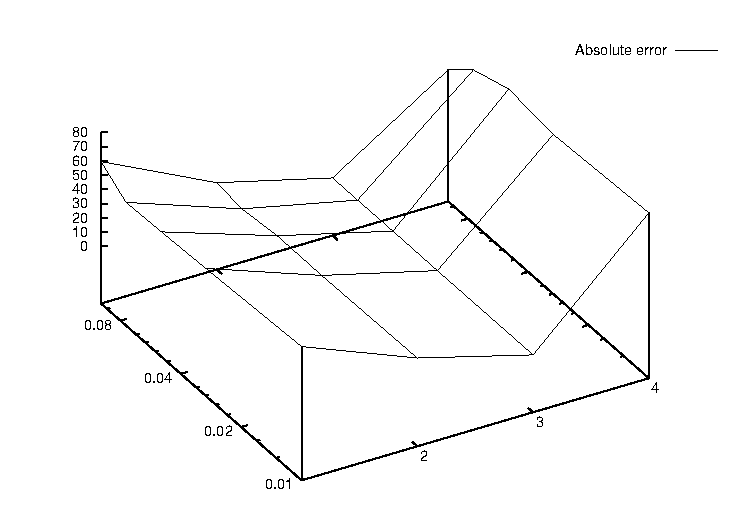
\includegraphics{graphics/svm_degree_epsilon.pdf}
\caption[Plot of the performance of a SVM]{The performance of a SVM (plot generated by {\tt gnuplot})}
\label{fig:svm_degree_epsilon_chart}
\end{figure}


\section{Support and tips}

\rapidminer is a complex data mining suite and provides a platform for a large
variety of process designs. We suggest that you work with some of the
building blocks described in this chapter and replace some operators and
parameter settings. You should have a look at the sample process definitions delivered
with \rapidminer and learn about other operators. However, the complexity of \rapidminer
might sometimes be very frustrating if you cannot manage to design the data
mining processes you want to. Please do not hesitate to use the user forum
and ask for help. You can also submit a support request. Both user forum
and support request tracker are available on our website
\begin{center}
\rapidminerurl
\end{center}
Beside this, we also offer services like support and consulting for our professional
users. Please contact us if you are interested in this form of professional support.

We conclude this chapter with some tips:
\begin{itemize}
\item You should make use of the automatic process validation available in
  the graphical user interface. This avoids a wrong process setup, missing
  parameter values, etc.
\item Work on a small subsample of your data during the process design and
  switch to the complete dataset if you are sure the process will properly
  run.
\item You do not have to write the attribute description files (XML) by
  hand. Just use the Attribute Editor of the GUI version or the configuration
  wizard of the \op{ExampleSource} operator.
\item Make use of breakpoints in the design phase. This helps to understand
  the data flow of \rapidminer and find potential problems, etc.
\item Start with small process setups and known building blocks and check if each
  new operator / operator chain performs in the way you have expected. 
\end{itemize}


\chapter{Operator reference}
\label{sec:operatorreference}

This chapter describes the built-in operators that come with
\rapidminer. Each operator section is subdivided into several parts:
\begin{enumerate}
\item The group and the icon of the operator.
\item An enumeration of the required input and the generated output
  objects. The input objects are usually consumed by the operator and
  are not part of the output. In some cases this behaviour can be changed by
  using a parameter \parval{keep\_\ldots}. Operators may also receive more
  input objects than required. In that case the unused input objects will be
  appended to the output and can be used by the next operator.
\item The parameters that can be used to configure the
  operator. Ranges and default values are specified. Required parameters
  are indicated by bullets (\textbullet) and optional parameters are
  indicated by an open bullet (\textopenbullet)
\item A list of values that can be logged using the
  \op{ProcessLog} operator (see page \pageref{sec:op:ProcessLog}).
\item If the operator represents a learning scheme, the capabilities
  of the learner are described. The learning capapabilities of most meta
  learning schemes depend on the inner learner.
\item If the operator represents an operator chain a short description of the
  required inner operators is given.
\item A short and a long textual description of the operator.
\end{enumerate}

The reference is divided into sections according to the operator groups known
from the graphical user interface. Within each section operators are
alphabetically listed.

% Notice that some operators extend the functionality of other
% operators. This is indicated by the word \textit{extends}. In this
% case, the operator inherits its parent's input and output classes,
% parameters, and values. Actually all operators extend \op{Operator} or
% \op{OperatorChain} but this is not indicated. 

% Some of the operators are \textit{abstract} and can not be used. They
% only serve as a superclass for other operators that have a common
% behavior or purpose. Abstract classes are set \textit{italic}.

\pagebreak







\chapter{Extending \rapidminer}
\label{sec:extending_rapidminer}

The core \rapidminer operators provide solutions for a large amount of usual
data mining applications. However, it is quite simple to write your own 
operators in order to extend \rapidminer. The platform provides the data management,
the nesting of operators, and the handling of optional and mandatory
parameters.

This chapter describes how to implement your own \rapidminer
operator\index{Operator} in Java. At least you should know the basic
concepts of this language to understand what we are doing here. All
necessary information about the \rapidminer classes can be found in the \rapidminer
API documentation which should be available on the \rapidminer homepage \rapidminerurl.


\section{Project structure}
In order to compile your own operators against \rapidminer, you must add
the file \filename{rapidminer.jar} and eventually some other \filename{jar} files in the
\filename{lib} directory of \rapidminer to your \commandline{CLASSPATH}. If
you downloaded the source version of \rapidminer, you should add the
\filename{build} directory (instead of \filename{rapidminer.jar}) to the
\commandline{CLASSPATH}. 

Using the source version of \rapidminer has the advantage that you can use
the \commandline{ant} buildfile. \commandline{ant} is a make-like
open source build tool for Java you can download from
\url{http://ant.apache.org}. The buildfile defines several useful
targets, among which is \commandline{build} which, as one may
easily guess, compiles all sources.

An Emacs JDE project file is also part of the source distribution. JDE
is the Java Development Environment for Emacs and turns Emacs into a
Java IDE. It can be downloaded from
\url{http://jdee.sunsite.dk}. On Unix platforms, Emacs is a widespread
editor but it also runs on Windows. It can be downloaded from
\url{http://www.gnu.org/software/emacs}.

There are also project files for Eclipse in the project folders. Eclipse is a 
powerful open-source IDE for Java which can be downloaded at \url{http://www.eclipse.org}.
It is also very easy to integrate the latest CVS version into Eclipse which is
described in detail at our web page\footnote{\rapidminerurl}.



\section{Operator skeleton}

The first step to do when implementing a new operator is to decide which class
must be extended. If your operator simply performs some action on its input and
delivers some output it should extend the class
\begin{center}
\java{com.rapidminer.operator.Operator}.
\end{center} 
If the operator shall be able to contain inner operators, it must
inherit from
\begin{center}
\java{com.rapidminer.operator.OperatorChain},
\end{center}
which itself extends \java{Operator}. Please refer to the API
documentation if there is a more specific subclass of
\java{Operator} which may serve your purpose. If your operator shall be a
learning scheme it might be useful to implement
\begin{center}
\java{com.rapidminer.operator.learner.Learner}
\end{center}
or extend
\begin{center}
\java{com.rapidminer.operator.learner.AbstractLearner}
\end{center}
though it does not need to. Similar interfaces and abstract operator classes
exists for other purposes too.

Now, there are some important things to specify about your operator.
These specifications will automatically be used for sanity checks, parameter
value checks, creation of GUI elements, and documentation. The following
methods must or should be overridden (if the operator does not inherit from
\java{Operator} directly, this may not be necessary):
\begin{enumerate}
\item One argument constructor: this constructor gets an object of the class 
  \java{OperatorDescription} which must be passed to the superclass by
  invoking \java{super(description)}.
\item \java{Class[] getInputClasses()}: Specifies the number and type of
  objects that are expected as input classes. Only classes that implement
  \java{com.rapidminer.operator.IOObject} may be passed between
  operators. Typical objects passed between operators include example sets,
  models, and performance vectors (see section \ref{sec:op:inandout}).
\item \java{Class[] getOutputClasses()}: Specifies the number and type of
  objects that are generated by this operator as output classes.
\item \java{List<ParameterType> getParameterTypes()}: Specifies the names and types
  of parameters that may be queried by this operator. Please make sure
  to add the parameter types to a \java{java.util.List} retrieved by a
  call to \java{super.get\-Pa\-ra\-me\-ter\-Types()}. The usage of subclasses of
  \java{ParameterType} for this purpose is described in
  sections~\ref{sec:op:adding_parameters} and the retrieval of
  parameter values is described in section~\ref{sec:op:getting_parameters}.
\item \java{IOObject[] apply()}: This is the main method that is
  invoked whenever the operator should perform its work. This method
  can query parameter values, input objects, and maybe call the
  \java{apply} methods of inner operators (in case of an operator chain). It
  returns an array of \java{IOObject}s as a result.\index{Operator!performing action}
  Please note that this method might throw an exception of type
  \java{OperatorException}.
\end{enumerate}

If your operator extends \java{OperatorChain} is must additionally implement
the following methods:
\begin{enumerate}
\item \java{int getMaxNumberOfInnerOperators()} and
  \java{getMin\-Num\-ber\-Of\-In\-ner\-Ope\-ra\-tors()}: these methods specify
  the maximum and minimum number of inner operators allowed for the operator
  chain. Return 0 and \java{Integer.MAX\_VALUE}, respectively for an unlimited
  number of inner operators.
\item \java{InnerOperatorCondition getInnerOperatorCondition()}: Operator
  chains have to implement this method. The delivered condition is used to
  perform checks if all inner operators can handle their input and deliver the
  necessary output. Several implementations for InnerOperatorCondition are
  available, please refer to the API documentation for details.
\end{enumerate}


Please have a look at the simple operator skeleton\index{Operator!skeleton}
showed in figure \ref{fig:operatorskeleton}. As described above, the operator
skeleton extends the class \java{Operator}.

\javafile{operatorskeleton.jav}{operatorskeleton}{Operator skeleton}{Operator skeleton}

The methods \java{getInputClasses()} and \java{getInputClasses()} do
not declare any input and output objects yet and so does the method
\java{getParameterTypes()}, which simply returns the parameters
declared by its superclass. According to these declarations, the
\java{apply()} method does nothing, but quietly returns an empty
array. The following sections describe, how you can fill these methods
with code.

\textit{Note:} Since version 3.0 of \rapidminer\ each operator must have an
one-argument constructor which must at least pass the given operator
description object to the superclass constructor. Please note that
during operator construction the method getParameterTypes() will be
invoked and must be fully functional, i.\,e. not depending on uninitialized
fields of the operator.

Finally, if your operator is implemented and you want to use it from
\rapidminer, you must declare the new operator class by adding a short entry
to an XML file. This is described in
section~\ref{sec:op:declaring_operators}.




\section{Useful methods for operator design}

Before we discuss an easy example for a self-written operator, the required methods are
described in detail. These methods enable you to declare a parameter, query a
parameter value, adding a \java{Value} which can be plotted by the
\op{PocessLog} operator and handling the in- and output of your operator.



\subsection{Defining parameters}
\label{sec:op:adding_parameters}

As we have seen above, the method \java{getParameterTypes()} can be used to
add parameters to your operator. Each parameter is described by a
\java{ParameterType} object, i.e. an object which contains the name, a small
description, and in case of a numerical parameter the range and default
value of this parameter. A new parameter type has to extend the class
\begin{center}
\java{com.rapidminer.parameter.ParameterType}
\end{center} 
In \rapidminer, for each simple data type a parameter type is
provided, e.g. for boolean values the type \java{ParameterTypeBoolean} or
\java{ParameterTypeInteger} for integers.
Table \ref{tab:op:parametertypes} shows all possible parameter types. Please
refer to the API documentation for details on constructing the different
parameter types.

Since the method \java{getParameterTypes()} returns a list of \java{ParameterType}s, your operator should
first invoke \java{super.getParameterTypes()} and add its parameter types to
the list which is returned by this method. In this way it is ensured that the
parameters of super classes can also be set by the user. Figure
\ref{fig:addingparameter} shows how a new integer parameter is added.

\javafile{addingparameter.jav}{addingparameter}{Adding a parameter}{Adding a parameter}

As you can see you create a new \java{ParameterTypeInteger} and add it to the
list. The first argument of the constructor is the name of the parameter which
will be used in the XML description files or in the GUI parameter
table. The second argument is a short description. This is used as tool tip
text when the mouse pointer stays on the parameter in the GUI for some seconds. For numerical
parameter types a range can be specified. The first number defines the minimum
value of this parameter, the second the maximum value. The last number is the
default value which is used when the user do not change this parameter in the
process setup.

Not every operator needs parameters. This is the reason why the method
\java{getParameterTypes()} is not abstract in Operator. You can simply ommit
the implementation of this method if your operator does not use any
parameters. However, you should notice that the method
\java{getParameterTypes()} is invoked by the super-constructor. You should
therefore not use global variables which are not initialized yet.


\newcolumntype{Y}{>{\small\raggedright\arraybackslash}X}
\newcolumntype{Z}{>{\small\tt\raggedright\arraybackslash}X}
\renewcommand{\tabularxcolumn}[1]{p{#1}}
\begin{table}[htbp]
  \begin{tabularx}{\linewidth}{|Z|Y|}
    \hline
    \textbf{Type}                  & \textbf{Description} \\
    \hline\hline
    ParameterTypeBoolean   & A boolean parameter. The defined value can be queried by
    \java{getParameterAsBoolean(key)}. \\
    \hline
    ParameterTypeCategory  & A category parameter which allows defined
    strings. The index of the chosen string can be queried by
    \java{getParameterAsInt(key)}. \\
    \hline
    ParameterTypeColor     & A parameter for colors. This is currently only
    used for user interface settings. The specified color can be queried by
    \java{getParameterAsColor(key)}. \\
    \hline
    ParameterTypeDirectory & A directory. The path to the chosen directory
    can be queried by \java{getParameterAsString(key)}. \\
    \hline
    ParameterTypeDouble    & A real valued parameter. The defined value can be queried by
    \java{getParameterAsDouble(key)}. \\
    \hline
    ParameterTypeFile      & A file. The path to the chosen file can be queried
    by \java{getParameterAsString(key)}.\\
    \hline
    ParameterTypeInt       & A integer parameter. The defined value can be queried by
    \java{getParameterAsInt(key)}. \\
    \hline
    ParameterTypeList      & A list of parameters of another parameter
    type. The defined list can be queried by \java{getParameterList(key)}. \\
    \hline
    ParameterTypePassword  & A password parameter. Passwords are masked with *
    in the GUI and queried by the system if the user has not specified the password in
    the process setup. The defined string can be queried by \java{getParameterAsString(key)}. \\
    \hline
    ParameterTypeString         & A simple string parameter. The defined value can be queried by
    \java{getParameterAsString(key)}. \\
    \hline
    ParameterTypeStringCategory & A category parameter which allows defined
    strings. Additionally the user can specify another string. The chosen
    string can be queried by \java{getParameterAsString(key)}. \\
    \hline
  \end{tabularx}
  \caption[Parameter types]{These parameter types can be added to your operator. Please refer
    to the API documentation for details on creation.}
  \label{tab:op:parametertypes}
\end{table}



\subsection{Getting parameters}
\label{sec:op:getting_parameters}

Now you can add  different parameter types to your operator. For each type 
\begin{center}
ParameterTypeXXX
\end{center}
a method \java{getParameterAsXXX()} is provided by the superclass
\java{Operator} unless another method is described in table
\ref{tab:op:parametertypes}\index{parameter}. All these methods return
an appropriate Java type, e.g. \java{double} for \java{getParameterAsDouble()}. 
Table~\ref{tab:op:parameters} shows the parameter getter methods of
the class \java{Operator} in detail.

The methods \java{getParameterAsXXX()} will throw an UndefinedParameterError
if the user has not defined a value for a non-optional parameter without
default value. Since this Error extends UserError which extends
OperatorException you should just throw these error out of your apply
method. A proper GUI message will be automatically created.

The List returned by \java{getParameterList(String)} contains
Object arrays of length 2. The first object is a key (String) and the second
the parameter value object, e.g. a Double for ParameterTypeDouble.


\newcolumntype{Y}{>{\small\raggedright\arraybackslash}X}
\newcolumntype{Z}{>{\small\tt\raggedright\arraybackslash}X}
\renewcommand{\tabularxcolumn}[1]{p{#1}}
\begin{table}[htbp]
  \begin{tabularx}{\linewidth}{|Z|Y|}
    \hline
    \textbf{Method}                  & \textbf{Description} \\
    \hline\hline
    getParameterAsBoolean(String key) & Returns a parameter and
    casts it to boolean.\\
    \hline
    getParameterAsColor(String key)   & Returns a parameter and
    casts it to Java Color.\\
    \hline
    getParameterAsDouble(String key)  & Returns a parameter and
    casts it to double. \\
    \hline
    getParameterAsFile(String key)    & Returns a parameter and
    casts it to a Java File.\\
    \hline
    getParameterAsInt(String key)   & Returns a parameter and
    casts it to int.\\
    \hline
    getParameterAsString(String key) & Returns a parameter and
    casts it to String.\\
    \hline
    getParameterList(String key) & Returns a parameter and casts
    it to a Java List. \\
    \hline
  \end{tabularx}
  \caption{Methods for obtaining parameters from {\tt Operator}}
  \label{tab:op:parameters}
\end{table}



\subsection{Providing \java{Value}s for logging}
\index{values!providing}

As you can see, the operator skeleton contains a one-argument
constructor which must pass the given description object to the
super-constructor. This is necessary for the automatic operator
creation with help of factory methods (see section
\ref{sec:integrating_rapidminer}). These constructors can also be used to declare
\java{Value}s which can be queried by an \op{ProcessLog} operator
(see \ref{sec:op:ProcessLog}). Each value you want to add must extend 
\begin{center}
\java{com.rapidminer.operator.Value}
\end{center}
and override the abstract method \java{getValue()}.
Figure \ref{fig:addvalues} shows how you can add some values in the constructor of
your operator. Note that usually non-static inner classes are used to
extend \java{Value}. These classes have access to private fields of
the operator and may, e.g. return the number of the current run, the
current performance or similar values.

\javafile{addvalues.jav}{addvalues}{Adding \java{Value}s to your Operator which
  can be queried by \op{ProcessLog}.}{Adding \java{Value}s to your Operator}

\emph{Note:} Please make sure that the only purpose of an operator's
constructor should be to add values and \emph{not} querying parameters or
perform other actions. Since the operator description and parameters will be
initialized after operator construction these type of actions will probably
not work and might cause exceptions.




\subsection{Input and output}
\label{sec:op:inandout}

As default, operators consume their input by using it. This is often a
useful behavior, especially in complex process definitions. 
For example, a learning operator consumes an example set to produce a
model and so does a cross validation to produce a performance value of
the learning method. To receive the input \java{IOObject} of a certain
class simply use
\begin{center}
\java{<T extends IOObject> T getInput(Class<T> class)}
\end{center}
This method delivers the first object of the desired class which is in the
input of this operator. By using generics it is already ensured that the
delivered object has the correct type and no cast is necessary. 
The delivered object is consumed afterwards
and thus is removed from input. If the operator alters this object, it
should return the altered object as output again. Therefore, you have
to add the object to the output array which is delivered by the
\java{apply()} method of the operator. You also have to declare it in
\java{getOutputClasses()}.
All input objects which are not used by your operator will be
automatically passed to the next operators. 

\emph{Note:} In versions before 3.4 it was necessary to cast the delivered
object to the correct type. This cast is no longer necessary.

In some cases it would be useful if the user can define if the input
object should be consumed or not. For example, a validation chain like
cross validation should estimate the performance but should also be
able to return the example set which is then used to learn the overall
model.
Operators can change the default behavior for input consumation and
a parameter will be automatically defined and queried. The default
behavior is defined in the method \java{getInputDescription(Class cls)} 
of operator and should be overriden in these cases. Please
note that input objects with a changed input description must not be
defined in \java{getOutputClasses()} and must not be returned at the
end of apply. Both is automatically done with respect to the value of
the automatically created parameter. Figure \ref{fig:inputdescription}
shows how this could be done. Please refer to the Javadoc comments of
this method for further explanations.

\javafile{inputdescription.jav}{inputdescription}{Changing the input handling behavior of your operator. In this case, example sets should be consumed per default but a parameter named \java{keep\_example\_set} will be automatically defined.}{Changing the input handling behavior of your operator}




\subsection{Generic Operators}
\label{sec:op:generic}

Sometimes a generic operator class should be implemented which should provide
more than one operator. In this case several operators can be declared to
\rapidminer (see section \ref{sec:op:declaring_operators}) with the same class but
different names. The subtype or name of an operator can be requested by
\java{getOperatorClassName()} which is a method of operator. Although this is very
similar to define the operator type with help of a parameter, subtypes can be
used in more subtile way: they can already be used to define the parameters and
therefore each subtype of an operator class may have other parameters. This
feature is used to provide a normal \rapidminer operator with different parameter
types for each Weka operator with the help of only one (short)
class. Please check the source code of the Weka learners for an example of a
generic operator.



\section{Example: Implementation of a simple operator}

After these technical preliminary remarks we set an example
which performs a very elementary task: It should write all examples of
an \ioobj{ExampleSet} into a file. First we consider that all we need as
input for this operator is an example set. Since we will not
manipulate it, we deliver the same example set as output. Therefore the methods
\java{getInputClasses()} and \java{get\-Out\-put\-Cla\-sses()} will only contain
one class: \java{com.rapidminer.example.ExampleSet}. If \ioobj{ExampleSet} is
not contained in the output of the former operator, your operator can not work
and \rapidminer\ will terminate at the beginning of the process. 

Your operator uses one parameter: A file where it should store the
examples. Therefore a \java{ParameterTypeFile} is added to the parameter
list. The third argument in the constructor indicates that this parameter is
mandatory.
Let us presume that your own operators are in the package
\java{my.new.operators}. Please have a look at the operator in figure
\ref{fig:examplesetwriter}, then we will explain the apply() function in detail.

\javafile{examplesetwriter.jav}{examplesetwriter}{Implementation of an
  example set writer}{Implementation of an example set writer}

The first line in \java{apply()} fetches the name of the file to
write the example set to. This method returns the value of the
parameter ``example\_set\_file'', if it is declared in the operator section
of the process configuration file. Since this parameter is mandatory
the process ends immediately with an error message if this parameter is not given.

We need the input example set to iterate through the examples and write them
to a file. We simply use the \java{getInput(ExampleSet.class)} method in order 
to get the desired input object (the example set). 

\emph{Note:} Please note that a cast to \java{ExampleSet} is not necessary. 
For \rapidminer versions before 3.4 a cast to the actual type has to be performed.

Then a stream to the specified file is opened
and an iterator over the examples is created. With this
\java{Iterator<Example>} you can pass through the examples of an example set
like the way you do with a \java{List} iterator. For each example the
values are written into the file and afterwards the stream to the file
is closed. Each operator can throw an \java{OperatorException} to the
calling operator, which would be done if any exception occurred during
writing the file. In this case the thrown exception is an \java{UserError}
which is used because writing presumably fails because the file is not
writable. We will discuss the error handling in section
\ref{sec:op:logservice}.

\emph{Note:} In versions before 3.4 the iterator was called \java{ExampleReader}.
Changing to the generic \java{Iterator<Example>} also allows for the nice new
for-loop introduced in Java 5.0: \java{for (Example e : exampleSet) \ldots}.

The last thing to do is creating a new array of 
{\tt IOObjects} which contains only the used \ioobj{ExampleSet} since no
additional output was produced.
The next section describes the iterating through an example set in detail,
then the exception concept will be explained.



\subsection{Iterating over an \ioobj{ExampleSet}}

\rapidminer\ is about data mining and one of the most frequent applications
of data mining operators is to iterate over a set of examples. This
can be done for preprocessing purposes, for learning, for applying a
model to predict labels of examples, and for many other tasks. We have seen
the mechanism in our example above and we will describe it below.

The way you iterate over an example set is very similar to the concept
of iterators, e.g. in terms of \java{Lists}. The methods which are provided
have the same signature as the methods of a Java \java{Iterator}. The first
thing you have to do is to create such an iterator. The following code 
snippet will show you how:

\javafile{examplereader.jav}{examplereader}{Creating and using an example
  iterator}{Creating and using an example iterator}

Assume \java{exampleSet} is a set of examples which we get from the input
of the operator. First of all, an iterator is created and then we traverse
through the examples in a loop. These iterators are backed up by different
implementations of the interface \java{ExampleReader}. The
classes \ioobj{ExampleSet}\index{ExampleSet},
\ioobj{ExampleReader}\index{ExampleReader}, and
\ioobj{Example}\index{Example} are provided within the package
\java{com.rapidminer.example}. Please check the \rapidminer\ API documentation to
see what else can be done with example sets and examples.



\subsection{Log messages and throw Exceptions}
\label{sec:op:logservice}

If you write your operator, you should make some logging messages
so\index{messages}\index{logging} that users can understand what your
operator is currently doing. It is especially reasonable to log error messages as
soon as possible. \rapidminer\ provides some methods to log the messages of
an operator. We distinguish between {\em log messages} and {\em
results}\index{results}. Of course you can write your results into the
normal log file specified in the process configuration file. But
the intended way to announce results of the process is to use a
\op{ResultWriter} (see section
\ref{sec:op:ResultWriter})\index{ResultWriter@{\op{ResultWriter\/}}} which writes each
currently available result residing in his input. For this purpose two classes
exist, a class \java{LogService} and a class
\java{ResultService}\index{LogService}\index{ResultService}. The latter
can be used by invoking the static method 
\begin{center}
\java{logResult(String result)}
\end{center}
or by simply using a \op{ResultWriter} as described above.

The class \java{com.rapidminer.tools.LogService} provides the static method 
\begin{center}
  \java{logMessage(String message, int verbosityLevel)}
\end{center}
to log text messages. Possible verbosity levels are \java{MINIMUM}, \java{IO},
\java{STATUS}, \java{INIT}, \java{WARNING}, \java{EXCEPTION}, \java{ERROR}, \java{FATAL}, and
\java{MAXIMUM} which are all public constant static fields of
\java{LogService}. The verbosity levels \java{IO} and \java{INIT} should \emph{not}
be used by operator developers. Normal log messages should be logged with
verbosity level \java{STATUS}.


\subsection{Operator exceptions and user errors}

The best way to abort the process because of an error is throwing an
\java{OperatorException}. If the error occurred due to an unforseen
situation, an instance of \java{OperatorException} should be
thrown. To ease bug tracking, it is useful to pass RuntimeExceptions
to the OperatorException constructor as the \java{cause} parameter.
If the error was caused by wrong usage of the operator, e.g. missing
files, or wrong parameter values, an instance of \java{UserError}
should be thrown. An error code referencing an error message in the
file \filename{resources/UserErrorMessages.properties} must be passed
to the constructor of a \java{UserError}. These messages are formatted
using an instance of \java{MessageFormat}. Index numbers in curly
braces are replaced by the arguments passed to the \java{UserError}
constructor. Please refer to the API documentation for construction
details.




\section{Building operator chains}

Now you can extend \rapidminer\ by writing operators which perform tasks on a
given input and deliver the input or additional output to a
surrounding operator. We have discussed the specifications to create
the operator in such a way that it can be nested into other
operators. But what we have not seen is the possibility to write your
own operator chain, i.e. operators which contain inner operators to
which input will be given and whose output is used by your
operator. What transmutes a simple operator to an operator chain is the
possibility to contain other inner operators.

The way you create an operator chain is straightforward: First your
operator does not directly extend \java{Operator} any longer, 
but \java{OperatorChain}\index{OperatorChain@{\op{OperatorChain\/}}}
instead. Since \java{OperatorChain} extends \java{Operator} itself you still have to
implement the methods discussed above. 


The second thing you have to do is to declare how many inner operators
your operator can cope with. Therefore every operator chain has to
overwrite two abstract methods from \java{OperatorChain}:
\index{Operator!inner}
\begin{center}
\java{int getMinNumberOfInnerOperators()}
\end{center}
and
\begin{center}
\java{int getMaxNumberOfInnerOperators()}
\end{center}
which returns the minimum and maximum number of inner operators. If
these numbers are equal, your operator chain must include exactly this number
of inner operators or \rapidminer\ will terminate at the beginning of an
process. 


There is another method which you have to implement:
\begin{center}
\java{InnerOperatorCondition getInnerOperatorCondition()}
\end{center}
This method delivers a condition about the inner operators. This condition should
ensure that the current process setup is appropriate and all inner
operators can be executed. Several implementations of
\java{InnerOperatorCondition} are available, please check the API for further
details. We will explain both methods in detail when we discuss the example in
section \ref{sec:operatorchainexample}.



\subsection{Using inner operators}

You can simply use inner operators via the method 
\begin{center}
\java{getOperator(int index)}
\end{center}
which delivers the inner operator with the given index. You can invoke the
\java{apply()} method of this operator yourself. The \java{apply()} method of the
superclass automatically performs the actions of the inner operators. \rapidminer\
takes care of the sequential execution.



\subsection{Additional input}
\label{sec:io_container}
But what if you want to add additional {\tt IOObjects} to the input of an
inner operator? A cross-validation operator for example, divides an
example set into subsets and adds certain subsets to the input of a
learning operator and others to the input of an operator chain which
includes a model applier and a performance evaluator. In this case your
operator has to consume the original {\tt IOObject} and add others to the
input of the inner operators.\index{Operator!input}

In section \ref{sec:op:inandout} we have seen how an operator can get
the input. This is consumed per default. If your operator should add a
certain {\tt IOObject} to the input of an inner operator it simply has
to call the \java{apply()} method of the inner operator in a way like
\begin{center}
\java{apply(getInput().append(new IOObject[] \{ additionalIO \}))}
\end{center}
or
\begin{center}
\java{apply(new InputContainer(new IOObject[] \{ additionalIO \}))}.
\end{center}
The method \java{getInput()} delivers the \rapidminer container which
provides the input and output objects of the
operators\footnote{\java{com.rapidminer.operator.IOContainer}}\index{IOContainer}.
You can add an array of additional {\tt IOObjects} using the \java{append()}
method. The latter variant ignores the input for the current operator
chain and produces a new input container for the child operators.

You should also use this method if you want to use the same {\tt IOObject} as
input for an inner operator several times, e.g. in a loop, or if you
want to add more than one {\tt IOObject} to the input of an inner operator.



\subsection{Using output}

Inner operators can produce output which your surrounding operator
must handle. The call of the \java{apply(IOContainer)} method of an inner
operator delivers a container like the one described above. You can
get the {\tt IOObjects} out of this container with some
\java{getter}-methods provided by this class. Figure
\ref{fig:innerop} shows the methods to append additional input for
the inner operator and getting specified output from the result of the
\java{apply()} method. The example set is split before into training and test
set\index{Operator!output}.

\javafile{innerop.jav}{innerop}{In- and output of an inner operator}{In- and output of an inner operator}

Mostly you do not need to do anything about adding additional input or
getting the output and \rapidminer\ will manage the in- and output for your
operator. Pay attention to the fact that you do not need to care about the
learned model: \rapidminer\ copes with the learned model for your model applier.




\section{Example 2: Implementation of an operator chain}
\label{sec:operatorchainexample}

The following example does not make much sense for data mining purposes, but
it demonstrates the implementation of an operator chain. Figure
\ref{fig:operatorchainexample} shows the complete code.

\javafile{operatorchainexample.jav}{operatorchainexample}{Example implementation of an operator chain.}{Example implementation of an operator chain.}

All methods inherited of \java{Operator} are implemented as described
above. Since this operator chain uses no parameters, the method
\java{getParameterTypes()} is not overwritten. This operator chain must have
at least one inner operator, the maximum number of inner operators is the
biggest integer which Java can handle. The method which returns the estimated
number of steps of this operator chain makes use of a method of the superclass
\java{OperatorChain}: \java{getNumberOfChildrenSteps()} returns the sum of all
children's steps. 

The purpose of this operator chain is described in the \java{apply()}
method. This operator expects an example set as input and clones it before it
uses the clone as input for each of the inner operators. The inner operators
must produce a performance vector. These vectors are averaged and then
returned.

The desired in- and output behaviours of inner operators must be described
with a condition object returned by the method
\java{getInnerOperatorCondition()}. In this example each inner operator should
be able to handle an example set and deliver a performance vector.






\section{Overview: the data core classes}
\label{sec:data_core}

It will be sufficient for many data mining purposes to iterate through
the example set. However, in some cases one must perform some more
complex changes of data or meta data. \rapidminer tries to hide the
internal data transformations for typical data mining purposes. It
uses a view mechanism to make a trade-off between efficient data
mining data transformations and the usage of memory. In this section
we discuss some basic concepts of the data handling in \rapidminer to
support users who want to write more complex operators.

\begin{figure}[thbp]
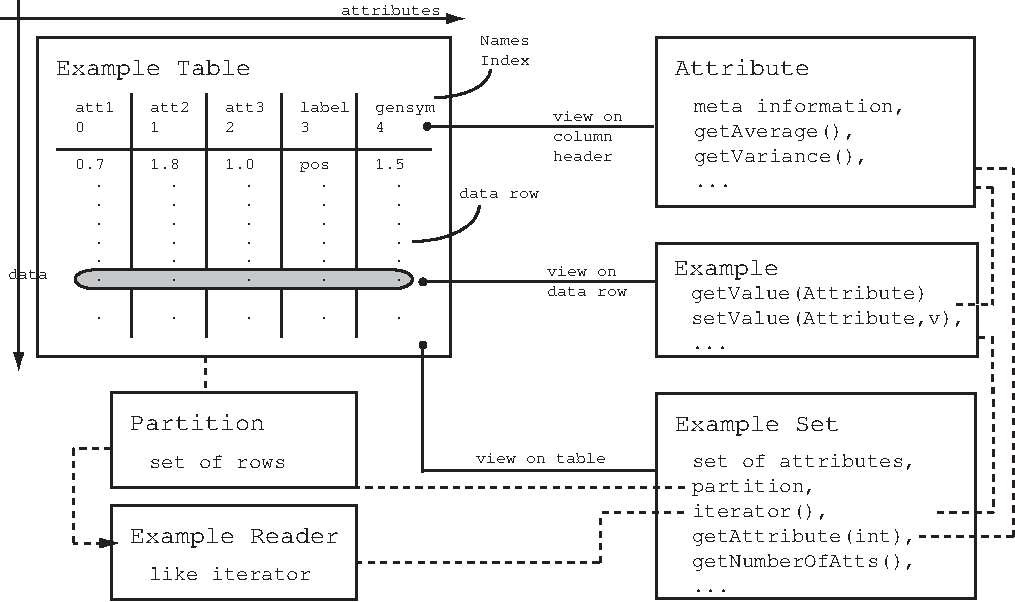
\includegraphics[width=\linewidth]{graphics/data_core.pdf}
\caption[Main classes for data handling]{The main classes used for
  data handling in \rapidminer. The central class is \java{ExampleTable}
  which keeps all data loaded and generated during
  processes. However, it is almost never directly used by operators.}
\label{fig:data_core}
\end{figure}


Figure \ref{fig:data_core} shows the main classes and interfaces which
are used for data handling in \rapidminer. The class \java{ExampleTable}
keeps all data which is loaded or generated during processes and
stores it in one table. The columns are defined by \java{Attribute}s,
which are used for two purposes: managing meta data about table columns
and referring to columns when one asks for the data in one cell. One
might say, that \java{Attribute} is a view on the header of a column
in the data table. Each row of the table is given by a
\java{DataRow}. Although the table is the central class for data
management, \rapidminer developers almost never use it directly. The other
classes shown in Figure \ref{fig:data_core} are used to encapsulate
the functionality and provide more convenient and secure ways to alter your
data.

Since \rapidminer is a data mining environment we often work on data. This
data is, as you know, given as \java{ExampleSet}s. Example sets
consist of a set of attributes and a partition. It is important to
understand, that example sets not keeps the data itself. That means
that you can copy an example set without copying the data. An example
set is merely a view on the example table\footnote{This is the reason
  why the index of an attribute in the example set is not in general
  equal to the index in the example table. To ask for the value of an
  attribute the \java{Attribute} object should always be used instead
  of the index.}.

An important method of example sets is the creation of an example
reader to iterate over the data. Depending whether the example set is
splitted with a partition, a particular instance of an example reader
is returned by the method \java{iterator()}. If only a
partition of examples is used, the returned example reader skips the
deselected examples. Applying weights
for attributes also requires a particular example reader, which
construct examples based on the weights. \rapidminer provides interfaces and
an adaptor concept for example sets to ensure the nestability of the
operators and the used example sets and readers.

The last important class in the data management of \rapidminer is
\java{Example} which is a view on a data row. Examples are constructed
on the fly by the current example reader of the used example set. The
current data row from the example table is used to back up the example
and weights are applied if a weighting or selection should be
applied. Since the indices of attributes in example sets and tables
must not be equal, the query for an attribute's value of an example
should always be performed with help of the attribute and not of it's
index.

Several subclasses exist for example set, example table, and example
reader. These subclasses provide different forms of data management
(main memory, database,\ldots) and views on your data. This concept ensures
data transparency for all operators and the nesting of operators. In
addition, new classes can be easily written to extend \rapidminer for
special purposes.





\section{Declaring your operators to \rapidminer}
\label{sec:op:declaring_operators}
At this point you know all the tricks to write your own operators and
the tool kit which is provided by \rapidminer for this purpose. The last
thing you have to do is to declare your operator to \rapidminer. Every
operator must comply with the following terms\index{Operator!declaring}:

\begin{description}
  \item[name] A meaningful name to specify the operator in a process 
    configuration file is required. The name must be unique.
  \item[class] The fully classified classname of your operator (must be in your
    java {\tt CLASSPATH} variable).
  \item[description] A short description of your operator and its task.
  \item[deprecation] A short description why your operator is deprecated and a short description of a workaround.
  \item[group] A name of a group. This may be your own group or one of the predefined
  \rapidminer group names.
  \item[icon] This is also optional but can be used to ease identification of
  the operator.
\end{description}

The definition of deprecation and icon are optional. If deprecation is omitted,
the operator is simply not regarded as deprecated - which is pretty much the default.
If icon is missing, the default icon for the operator group is used.
To link these description parts to one another you have to specify them in a
operator description file.
Every entry holds for one
operator and they are written like the ones in figure
\ref{fig:operators}. We assume that you save these descriptions in a file
named 'operators.xml'.

\examplefile{operators.xml}{operators}{Declaring operators to \rapidminer}

Additionally to simple operator entries you can specify one or more operator
factory classes which must implement the interface
\begin{center}
\java{com.rapidminer.tools.GenericOperatorFactory}.
\end{center}
This is especially useful if you want to provide more than one operator for
each class by working with operator subtypes. This is the preferred way to add 
generic operators with one class but more than subtype or operator name.

In order to use your operators with \rapidminer\ you have to add them to your {\tt
  CLASSPATH} variable. Then you can start \rapidminer\ with the option 
\begin{center}
\java{-Drapidminer.operators.additional=path/to/your/operators.xml}
\end{center}
Please edit your start scripts and add the parameter to the line which starts
\rapidminer\ or start \rapidminer\ manually with a call like

\java{java} \\
\java{-cp \$RAPIDMINER\_HOME/lib/rapidminer.jar:your/class/path} \\
\java{-Drapidminer.home=\$RAPIDMINER\_HOME} \\
\java{-Drapidminer.operators.additional=path/to/your/operators.xml} \\
\java{com.rapidminer.gui.RapidMinerGUI}

Your new operators should be available now and can be chosen in the GUI. More
than one additional operator description file can be specified by making use
of the system dependent path separator, for unix systems for example with 

\java{-Drapidminer.operators.additional=my\_operators.xml:other\_ops.xml} \\








\section{Packaging plugins}
\index{plugins!authoring}
\label{sec:plugins_packaging}
If you want to make your operators available for download, you can easily
create plugins.
\begin{enumerate}
\item Compile your Java sources.
\item Create a file named \filename{operators.xml} as described above
\item Create a jar archive using the \commandline{jar} command that comes with the
  JDK. The archive must contain your operator class files and all classes they
  depend on. The file \filename{operators.xml} must go into the
  \filename{META-INF} directory of the archive.
\item If desired, create a file named \filename{ABOUT.NFO} and add it
  to the \filename{META-INF} directory of the jar file.
\item IMPORTANT: You have to use a \filename{Manifest} file in the Jar archive.
  In this manifest file the entry \java{RapidMiner-Type} with the value 
  \java{RapidMiner\_Plugin} has to be used in order to make this Jar archive
  to a valid RapidMiner plugin (since version 4.2)! Additionally, the entries
  Implementation-Title, Implementation-Version, Implementation-Vendor,
  Implementation-URL, \rapidminer-Version, and Plugin-Dependencies will be evaluated
  by \rapidminer. \rapidminer-Version defines the minimum \rapidminer version which is needed for
  this plugin. Plugin-Dependencies must have the form \\
  plugin\_name1 [plugin\_version1] \# \ldots \# plugin\_nameM [plugin\_versionM]
\item You can include GUI icons for your operators within the
  jar file. If you set the \tag{icon} attribute of the \tag{<operator>} tag
  in the \filename{operators.xml} file to ``foo'', \rapidminer will look for a
  file named \filename{op\_foo.gif} in the directory
  \filename{com/rapidminer/resources/icons/groups/24} or in the directory 
  \filename{com/rapidminer/resources/icons/operators/24} of the jar file.
\item Copy the archive into \filename{lib/plugins} directory. If you like, also put
  it on your website or send it to us. Since \rapidminer is licensed under the GNU
  General Public License you have to develop your plugins as opensource
  software and you have to make it available for the \rapidminer community. If this
  is not possible for any reasons, e.g. because the development of the plugin
  was done for commercial purposes, you should contact us for a special
  commercial version of \rapidminer.
\end{enumerate}
Hint: If your plugin depends on external libraries, you do not have to
package these into one archive. You can reference the libraries using a
\commandline{Class-Path} entry in your jar \filename{Manifest} file.
For information on installation of plugins, please refer to
section~\ref{sec:plugins_installing}.




\section{Documentation}
The operator reference chapter of the  \LaTeX{} \rapidminer tutorial is
generated using the Javadoc class comments of the operator source
code. Therefore some additional Javadoc tags can be used. 
\begin{description}
\item[@rapidminer.xmlclass] The classname given in the
  \filename{operators.xml} if different from the classname.
\item[@rapidminer.index] For \LaTeX output generate an index entry for the
  tutorial referring to the description of this operator.
\item[@rapidminer.reference] A BibTeX key that will be used to generate a
  HTML bibliography entry. Ignored for \LaTeX{} output.
\item[@rapidminer.cite] Inline tag. For \LaTeX{} output generate a citation. For HTML
  output, simply print the key.
\item[@rapidminer.ref] Inline tag. For \LaTeX{} output generate a reference
  to a tutorial section, for HTML simply print the reference name.
\item[@rapidminer.xmlinput] The text of this tag must consist of three
  strings separated by a pipe symbol ("$|$"). The first string must be
  a filename, the second must be a label, and the third must be a
  caption for a figure. The file specified will be input both in HTML
  and \LaTeX{} documentation.
\end{description}
Please refer to the API documentation of the class
\begin{center}
com.rapidminer.docs.DocumentationGenerator
\end{center}
to learn how the documentation for your operators can automatically created
from your Java source code and Javadoc comments.
 


\section{Non-Operator classes}

Some operators, like \op{PerformanceEvaluator} and the
\op{ExampleFilter}, have parameters that let you specify
implementations of certain interfaces that will solve simple
subtasks, e.g. determining which of two performance vectors is
preferable, or which examples to remove from an example set. Those classes
must be specified with the fully qualified classname. If you want to implement
such an interface, you simply have to add the implementation to your classpath
and declare it to the operator. Of course it is also possible to add these
implementations to your plugin.


\section{Line Breaks}

In order to ensure platform compatibility you should never use $\backslash n$ in 
your code. Line breaks should always be created with help of the methods 
\begin{center}
\java{com.rapidminer.tools.Tools.getLineSeparator()}
\end{center}
for a single line break and
\begin{center}
\java{com.rapidminer.tools.Tools.getLineSeparators(int)}
\end{center}
for multiple line breaks.



\section{GUI Programming}

If you want to create visualizations of models or other output types
of your operators you might be interested to stick to the \rapidminer
look and feel guidelines. There are several things which should be considered 
for GUI programming:
\begin{itemize}
\item Use \java{ExtendedJTable} instead of \java{JTable}
\item Use \java{ExtendedJScrollBar} instead of \java{JScrollBar}
\item Use only the colors defined as constants in \java{SwingTools}
\end{itemize}



\chapter{Integrating \rapidminer into your application}
\label{sec:integrating_rapidminer}

\rapidminer can easily be invoked from other Java applications. 
You can both read process configurations from xml
\java{File}s or \java{Reader}s, or you can construct \java{Process}es
by starting with an empty process and adding \java{Operator}s
to the created \java{Process} in a tree-like manner. Of course you can also
create single operators and apply them to some input objects, e.g. learning a
model or performing a single preprocessing step. However, the creation of
processes allows \rapidminer to handle the data management and process
traversal. If the operators are created without beeing part of an process,
the developer must ensure the correct usage of the single operators himself.


\section{Initializing \rapidminer}

Before \rapidminer can be used (especially before any operator can be created),
\rapidminer has to be properly initialized.
The method 
\begin{center}
\java{RapidMiner.init()}
\end{center}
must be invoked before the \java{OperatorService} can be used to create operators. 
Several other initialization methods for \rapidminer exist, please make sure that you 
invoke at least one of these. If you want to configure the initialization of \rapidminer
you might want to use the method
\begin{center}
\begin{verbatim}
RapidMiner.init(InputStream operatorsXMLStream, 
			    File pluginDir, 
			    boolean addWekaOperators, 
			    boolean searchJDBCInLibDir, 
			    boolean searchJDBCInClasspath, 
			    boolean addPlugins)
\end{verbatim}
\end{center}
Setting some of the properties to false (e.g. the loading of database drivers or of 
the Weka operators might drastically improve the needed runtime during start-up. 
If you even want to use only a subset of all available operators you can provide a 
stream to a reduced operator description (operators.xml). If the parameter
\java{operatorsXMLStream} is null, just all core operators are used. Please
refer to the API documentation for more details on the initialization of \rapidminer.

You can also use the simple method \java{RapidMiner.init()} and configure the 
settings via this list of environment variables:
\begin{itemize}
\item \texttt{rapidminer.init.operators} (file name)
\item \texttt{rapidminer.init.plugins.location} (directory name)
\item \texttt{rapidminer.init.weka} (boolean)
\item \texttt{rapidminer.init.jdbc.lib} (boolean)
\item \texttt{rapidminer.init.jdbc.classpath} (boolean)
\item \texttt{rapidminer.init.plugins} (boolean)
\end{itemize}


	 
\section{Creating Operators}

It is important that operators are
created using one of the \java{createOperator(...)} methods of
\begin{center}
\java{com.rapidminer.tools.OperatorService}
\end{center} 
Table~\ref{tab:op:operator_creation} shows the different factory methods for
operators which are provided by OperatorService. Please note that few operators
have to be added to a process in order to properly work. Please refer 
to section \ref{sec:single_operators} for more details on using single operators and 
adding them to a process.


\newcolumntype{Y}{>{\small\raggedright\arraybackslash}X}
\newcolumntype{Z}{>{\small\tt\raggedright\arraybackslash}X}
\renewcommand{\tabularxcolumn}[1]{p{#1}}
\begin{table}[htbp]
  \begin{tabularx}{\linewidth}{|Z|Y|}
    \hline
    \textbf{Method}                  & \textbf{Description} \\
    \hline\hline
    createOperator(String name)      & Use this method for the creation of an
    operator from its name. The name is the name which is defined
    in the \filename{operators.xml} file and displayed in the GUI. \\
    \hline
    createOperator(Operator\-Description description) & Use this method for the creation of an
    operator whose OperatorDescription is already known. Please refer to the
    \rapidminer API. \\
    \hline
    createOperator(Class clazz) & Use this method for the creation of an
    operator whose Class is known. This is the recommended method for the
    creation of operators since it can be ensured during compile time
    that everything is correct. However, some operators exist which do not 
    depend on a particular class (e.g. the learners derivced from the Weka
    library) and in these cases one of the other methods must be used. \\
    \hline
  \end{tabularx}
  \caption[Operator factory methods of OperatorService]{These methods should
    be used to create operators. In this way it is ensured that the operators
    can be added to processes and properly used.}
  \label{tab:op:operator_creation}
\end{table}




\section{Creating a complete process}

Figure~\ref{fig:createops} shows a detailed example for the \rapidminer API to create
operators and setting its parameters.

\javafile{createops.jav}{createops}{Creation of new operators and setting up
  an process from your application}{Creation of new operators and
  process setup}

We can simply create a new process setup via \java{new Process()} and
add operators to the created process. The root of the process' operator tree 
is queried by \java{process.getRootOperator()}. Operators are added like children to a
parent tree. For each operator you have to
\begin{enumerate}
\item create the operator with help of the OperatorService,
\item set the necessary parameters,
\item add the operator at the correct position of the operator tree of the process.
\end{enumerate}

After the process was created you can start the process via
\begin{center}
\java{process.run()}. 
\end{center}
If you want to provide some initial input you can also use the method
\begin{center}
\java{process.run(IOContainer)}.
\end{center}
If you want to use a log file you should set the parameter \java{logfile}
of the process root operator like this 
\begin{center}
\java{process.getRootOperator().setParameter(
ProcessRootOperator.PARAMETER\_LOGFILE, 
filename
)}
\end{center}
before the run method is invoked. If you want also to keep the global 
logging messages in a file, i.e. those logging messages which are not associated 
to a single process, you should also invoke the method
\begin{center}
\java{LogService.initGlobalLogging(
OutputStream out, 
int logVerbosity
)}
\end{center}
before the run method is invoked.


If you have already defined a process configuration file, for example
with help of the graphical user interface, another very simple way of
creating a process setup exists. Figure~\ref{fig:rapidminer_from_external} shows how
a process can be read from a process configuration file. 
Just creating a process from a file (or stream) is a very simple way to 
perform processes which were created with the graphical user interface 
beforehand.


\javafile{RapidMinerFromExternal.jav}{rapidminer_from_external}{Using complete \rapidminer
  processes from external programs}{Using a \rapidminer process from external
  programs}

As it was said before, please ensure that \rapidminer was properly initialized by one of the 
init methods presented above.



\section{Using single operators}
\label{sec:single_operators}

The creation of a \java{Process} object is the intended way of performing a complete
data mining process within your application. For small processes like a
single learning or preprocessing step, the creation of a complete process
object might include a lot of overhead. In these cases you can easily manage the
data flow yourself and create and use single operators.

The data flow is managed via the class \java{IOContainer} (see section
\ref{sec:io_container}). Just create the operators you want to use, set
necessary parameters and invoke the method \java{apply(IOContainer)}. 
The result is again an \java{IOContainer} which can deliver the desired output
object. Figure~\ref{fig:rapidminer_from_external2} shows a small programm which loads
some training data, learns a model, and applies it to an unseen data set.

\javafile{RapidMinerFromExternal2.jav}{rapidminer_from_external2}{Using single \rapidminer
  operators from external programs}{Using \rapidminer operators from external
  programs}

Please note that using an operator without an surrounding process is only
supported for operators not directly depending on others in an process
configuration. This is true for almost all operators available in \rapidminer. There
are, however, some exceptions: some of the meta optimization operators (e.g. 
the parameter optimization operators) and the ProcessLog operator only work
if they are part of the same process of which the operators should be optimized 
or logged respectively. The same applies for the MacroDefinition operator which
also can only be properly used if it is embedded in a \java{Process}. Hence, 
those operators cannot be used without a Process and an error will occur.

Please note also that the method 
\begin{center}
\java{RapidMiner.init()}
\end{center}
or any other \java{init()} taking some parameters must be invoked before the 
\java{OperatorService} can be used to create operators (see above).


\section{\rapidminer as a library}

If \rapidminer is separately installed and your program uses the \rapidminer classes
you can just adapt the examples given above. However, you might also want
to integrate \rapidminer into your application so that users do not have to download
and install \rapidminer themself. In that case you have to consider that
\begin{enumerate}
\item \rapidminer needs a \filename{rapidminerrc} file in \filename{rapidminer.home/etc}
  directory
\item \rapidminer might search for some library files located in the directory
  \filename{rapidminer.home/lib}.
\end{enumerate}
For the Weka jar file, you can define a
system property named \java{rapidminer.weka.jar} which defines where the Weka jar
file is located. This is especially useful if your application already
contains Weka. However, you can also just omit all of the library jar files,
if you do not need their functionality in your application. 
\rapidminer will then just work without this additional functionality, for example,
it simply does not provide the Weka learners if the weka.jar library was omitted.



\section{Transform data for \rapidminer}

Often it is the case that you already have some data in your application on which 
some operators should be applied. In this case, it would be very annoying to write
your data into a file, load it into \rapidminer with an ExampleSource operator and apply
other operators to the resulting ExampleSet. It would therefore be a nice feature
if it would be possible to directly use your own application data as input. 
This section describes the basic ideas for this approach.

As we have seen in Section \ref{sec:data_core}, all data is stored in a central data 
table (called \java{ExampleTable}) and one or more views on this table (called \java{ExampleSet}s) 
can be created and will be used by operators. Figure \ref{fig:creating_example_tables} 
shows how this central \java{ExampleTable} can be created. 

\javafile{creatingexampletables.jav}{creating_example_tables}{The complete code for creating a memory based ExampleTable}{The complete code for creating a memory based ExampleTable}

First of all, a list containing
all attributes must be created. Each \java{Attribute} represents a column in the final example 
table. We assume that the method \java{getMyNumOfAttributes()} returns the number of regular 
attributes. We also assume that all regular attribute have numerical type. We create
all attributes with help of the class \java{AttributeFactory} and add them to the attribute list. 

For example tables, it does not matter if a specific column (attribute) is a 
special attribute like a classification label or just a regular attribute which is used
for learning. We therefore just create a nominal classification label and add it to
the attribute list, too.

After all attributes were added, the example table can be created. In this example we create a 
\java{MemoryExampleTable} which will keep all data in the main memory. The attribute list is given
to the constructor of the example table. One can think of this list as a description of the
column meta data or column headers. At this point of time, the complete table is empty, i.e.
it does not contain any data rows.

The next step will be to fill the created table with data. Therefore, we create a DataRow 
object for each of the \java{getMyNumOfRows()} data rows and add it to the table. 
We create a simple double array
and fill it with the values from your application. In this example, we assume that the method
\java{getMyValue(d,a)} will deliver the value for the $a$-th attribute of the $d$-th data row.
Please note that the order of values and the order of attributes added to the attribute list
must be the same!

For the label attribute, which is a nominal classification value, we have to map the \java{String}
delivered by \java{getMyClassification(d)} to a proper double value. This is done with the method
\java{mapString(String)} of \java{Attribute}. This method will ensure that following mappings 
will always produce the same double indices for equal strings.

The last thing in the loop is to add a newly created \java{DoubleArrayDataRow} to the example table. 
Please note that only MemoryExampleTable provide a method \java{addDataRow(DataRow)}, other
example tables might have to initialized in other ways.


The last thing which must be done is to produce a view on this example table. Such views are called
\java{ExampleSet} in \rapidminer. The creation of these views is done by the method 
\java{createCompleteExampleSet(label, null, null, null)}. The resulting example set
can be encapsulated in a \java{IOContainer} and given to operators.

\paragraph{Remark:}
Since Attribute, DataRow, ExampleTable, and ExampleSet are all interfaces, you can of course implement
one or several of these interfaces in order to directly support \rapidminer with data even without
creating a MemoryExampleTable.



\chapter{Acknowledgements}
\label{sec:Acknowledgements}

We thank SourceForge\footnote{\url{http://sourceforge.net/}} for providing a
great platform for open-source development.

We are grateful to the developers of
Eclipse\footnote{\url{http://www.eclipse.org}},
Ant\footnote{\url{http://ant.apache.org}}, and
JUnit\footnote{\url{http://www.junit.org}} for making these great
open-source development environments available.

We highly appreciate the operators and extensions written by several external
contributors. Please check our website for a complete list of authors.

We thank the Weka\footnote{\url{http://www.cs.waikato.ac.nz/ml/weka/}} developers for
providing an open source Java archive with lots of great machine learning
operators.

We are grateful to Stefan R\"uping for providing his implementation of a
support vector machine\footnote{\url{http://www-ai.informatik.uni-dortmund.de/SOFTWARE/MYSVM/}}.

We thank Chih-Chung Chang and Chih-Jen Lin for their SVM implementation
LibSVM\footnote{\url{http://www.csie.ntu.edu.tw/cjlin/libsvm/}}.

We would like to thank Stefan Haustein for providing his library
\java{kdb}\footnote{\url{http://www.me.objectweb.org/}}, which we use for several
input formats like dBase and BibTeX.

Thanks to the users of \rapidminer. Your comments help to improve \rapidminer for
both end users and data mining developers.



\begin{appendix}

\chapter{Regular expressions}
\label{sec:regular_expressions}

Regular expressions are a way to describe a set of strings based on common
characteristics shared by each string in the set. They can be used as a tool
to search, edit or manipulate text or data. Regular expressions range from
being simple to quite complex, but once you understand the basics of how
they're constructed, you'll be able to understand any regular expression.

In \rapidminer several parameters use regular expressions, e.g. for the definition
of the column separators for the ExampleSource operator or for the feature
names of the FeatureNameFilter. This chapter gives an
overview of all regular expression constructs available in \rapidminer. These are
the same as the usual regular expressions available in Java. Further
information can be found at
\begin{center}
\url{http://java.sun.com/docs/books/tutorial/essential/regex/index.html}.
\end{center}



\section{Summary of regular-expression constructs}


\begin{longtable}{|p{3cm}|p{8cm}|}

\hline
 & \\
\textbf{Construct} & \textbf{Matches} \\
 & \\
\hline
\endhead

\hline
\endfoot

\multicolumn{2}{|l|}{\textbf{}}\\
\multicolumn{2}{|l|}{\textbf{Characters}}\\
\hline
x &	The character x \\
$\backslash$$\backslash$ & The backslash character \\
$\backslash$0n & The character with octal value 0n (0 $<$= n $<$= 7) \\
$\backslash$0nn & The character with octal value 0nn (0 $<$= n $<$= 7) \\
$\backslash$0mnn & The character with octal value 0mnn (0 $<$= m $<$= 3, 0 $<$= n $<$= 7) \\
$\backslash$xhh & The character with hexadecimal value 0xhh \\
$\backslash$uhhhh & The character with hexadecimal value 0xhhhh \\
$\backslash$t & The tab character ('$\backslash$u0009') \\
$\backslash$n & The newline (line feed) character ('$\backslash$u000A') \\
$\backslash$r &	The carriage-return character ('$\backslash$u000D') \\
$\backslash$f &	The form-feed character ('$\backslash$u000C') \\
$\backslash$a &	The alert (bell) character ('$\backslash$u0007') \\
$\backslash$e &	The escape character ('$\backslash$u001B') \\
$\backslash$cx & The control character corresponding to x \\
\hline
\multicolumn{2}{|l|}{\textbf{}}\\
\multicolumn{2}{|l|}{\textbf{Character classes}}\\
\hline
{[}abc{{]}}& a, b, or c (simple class) \\
{[}\textasciicircum abc{{]}} & Any character except a, b, or c (negation) \\
{[}a-zA-Z{]} & a through z or A through Z, inclusive (range) \\
{[}a-d{[}m-p{]}{]} & a through d, or m through p: {[}a-dm-p{]} (union) \\
{[}a-z\&\&{[}def{]}{]} & d, e, or f (intersection) \\
{[}a-z\&\&{[}\textasciicircum bc{]}{]} & a through z, except for b and c: {[}ad-z{]} (subtraction) \\
{[}a-z\&\&{[}\textasciicircum m-p{]}{]} & a through z, and not m through p: {[}a-lq-z{]}(subtraction) \\
\hline
\multicolumn{2}{|l|}{\textbf{}}\\
\multicolumn{2}{|l|}{\textbf{Predefined character classes}}\\
\hline
. & Any character (may or may not match line terminators) \\
$\backslash$d &	A digit: {[}0-9{]} \\
$\backslash$D &	A non-digit: {[}\textasciicircum0-9{]} \\
$\backslash$s &	A whitespace character: {[} $\backslash$t$\backslash$n$\backslash$x0B$\backslash$f$\backslash$r{]} \\
$\backslash$S &	A non-whitespace character: {[}\textasciicircum$\backslash$s{]} \\
$\backslash$w &	A word character: {[}a-zA-Z\_0-9{]} \\
$\backslash$W &	A non-word character: {[}\textasciicircum$\backslash$w{]} \\
\hline
\multicolumn{2}{|l|}{\textbf{}}\\
\multicolumn{2}{|l|}{\textbf{POSIX character classes (US-ASCII only)}}\\
\hline
$\backslash$p\{Lower\} & A lower-case alphabetic character: {[}a-z{]} \\
$\backslash$p\{Upper\} & An upper-case alphabetic character: {[}A-Z{]} \\
$\backslash$p\{ASCII\} & All ASCII: {[}$\backslash$x00-$\backslash$x7F{]} \\
$\backslash$p\{Alpha\} & An alphabetic character:{[}$\backslash$p\{Lower\}$\backslash$p\{Upper\}{]} \\
$\backslash$p\{Digit\} & A decimal digit: {[}0-9{]} \\
$\backslash$p\{Alnum\} & An alphanumeric  character:{[}$\backslash$p\{Alpha\}$\backslash$p\{Digit\}{]} \\
$\backslash$p\{Punct\} & Punctuation: One of !"\#\$\%\&'()*+,-./:;$<$=$>$?@{[}$\backslash${]}\textasciicircum\_ $\grave{}$\{|\}$\sim$ \\
$\backslash$p\{Graph\} & A visible character: {[}$\backslash$p\{Alnum\}$\backslash$p\{Punct\}{]} \\
$\backslash$p\{Print\} & A printable character: {[}$\backslash$p\{Graph\}{]} \\
$\backslash$p\{Blank\} & A space or a tab: {[} $\backslash$t{]} \\
$\backslash$p\{Cntrl\} & A control character:  {[}$\backslash$x00-$\backslash$x1F$\backslash$x7F{]} \\
$\backslash$p\{XDigit\} & A hexadecimal digit: {[}0-9a-fA-F{]} \\
$\backslash$p\{Space\} & A whitespace character: {[}  $\backslash$t$\backslash$n$\backslash$x0B$\backslash$f$\backslash$r{]} \\
\hline
\multicolumn{2}{|l|}{\textbf{}}\\
\multicolumn{2}{|l|}{\textbf{Classes for Unicode blocks and categories}}\\
\hline 
$\backslash$p\{InGreek\} & A character in the Greek block (simple block) \\
$\backslash$p\{Lu\} & An uppercase letter (simple category) \\
$\backslash$p\{Sc\} & A currency symbol \\
$\backslash$P\{InGreek\} & Any character except one in the Greek block (negation) \\
{[}$\backslash$p\{L\}\&\&{[}\textasciicircum$\backslash$p\{Lu\}{]}{]} & Any letter except an uppercase letter (subtraction) \\
\hline
\multicolumn{2}{|l|}{\textbf{}}\\
\multicolumn{2}{|l|}{\textbf{Boundary matchers}}\\
\hline 
\textasciicircum & The beginning of a line \\
\$ & The end of a line \\
$\backslash$b &	A word boundary \\
$\backslash$B &	A non-word boundary \\
$\backslash$A &	The beginning of the input \\
$\backslash$G &	The end of the previous match \\
$\backslash$Z &	The end of the input but for the final terminator, if any \\
$\backslash$z &	The end of the input \\
\hline
\multicolumn{2}{|l|}{\textbf{}}\\
\multicolumn{2}{|l|}{\textbf{Greedy quantifiers}}\\
\hline  
X? & X, once or not at all \\
X* & X, zero or more times \\
X+ & X, one or more times \\
X\{n\} & X, exactly n times \\
X\{n,\} & X, at least n times \\
X\{n,m\} & X, at least n but not more than m times \\
\hline
\multicolumn{2}{|l|}{\textbf{}}\\
\multicolumn{2}{|l|}{\textbf{Reluctant quantifiers}}\\
\hline   
X?? &	X, once or not at all \\
X*? &	X, zero or more times \\
X+? &	X, one or more times \\
X\{n\}? &	X, exactly n times \\
X\{n,\}? & X, at least n times \\
X\{n,m\}? & X, at least n but not more than m times \\
\hline
\multicolumn{2}{|l|}{\textbf{Logical operators}}\\
\hline    
XY & X followed by Y \\
X|Y & Either X or Y \\
(X) & X, as a capturing group \\
\hline
\multicolumn{2}{|l|}{\textbf{}}\\
\multicolumn{2}{|l|}{\textbf{Back references}}\\
\hline 
$\backslash$n & Whatever the $n$-th capturing group matched \\
\hline
\multicolumn{2}{|l|}{\textbf{}}\\
\multicolumn{2}{|l|}{\textbf{Quotation}}\\
\hline    
$\backslash$ & Nothing, but quotes the following character \\
$\backslash$Q & Nothing, but quotes all characters until $\backslash$E \\
$\backslash$E & Nothing, but ends quoting started by $\backslash$Q \\
\hline
\multicolumn{2}{|l|}{\textbf{}}\\
\multicolumn{2}{|l|}{\textbf{Special constructs (non-capturing)}}\\
\hline    
(?:X) & X, as a non-capturing group \\
(?idmsux-idmsux) & Nothing, but turns match flags on - off \\
(?idmsux-idmsux:X) & X, as a non-capturing group with the given flags on - off \\
(?=X) & X, via zero-width positive lookahead \\
(?!X) & X, via zero-width negative lookahead \\
(?$<$=X) & X, via zero-width positive lookbehind \\
(?$<$!X) & X, via zero-width negative lookbehind \\
(?$>$X) & X, as an independent, non-capturing group \\
\hline
\end{longtable}


\end{appendix}

%%  =====  Literaturverzeichnis  =====
%%
\bibliographystyle{plain} 
\bibliography{RapidMinerTutorial}

\printindex

\end{document}
